\chapter{The Primes}\label{ch:primes}

\begin{chapterintro}
In chemistry every substance is built from a short list of atoms, and every molecule has a definite recipe: water is two hydrogens and one oxygen, never anything else. Whole numbers have their own atoms. Every whole number larger than 1 is either one of these atoms (a \emph{prime}) or a product of them, and the recipe is unique: $60$ is $2\cdot2\cdot3\cdot5$ and nothing else. This chapter is about those atoms. We define them, prove that the recipe always exists and is unique, prove that there is no last prime, learn to list them with a two-thousand-year-old algorithm, and then ask the question that leads directly to the Riemann zeros: \emph{how many} primes are there below a given size?

The answer, the prime number theorem, says that near a large number $x$ roughly one number in $\log x$ is prime. Along the way we meet two weighted ways of counting primes, the von Mangoldt function $\Lambda(k)$ and Chebyshev's function $\psi(x)$, which turn out to be the natural language of the zeta function. We end by explaining why the logarithm $\log p$, rather than $p$ itself, is the natural ``size'' of a prime.

\emph{Where this shows up in the paper.} The paper's arithmetic predictor, Eq.~(4) of \cite{soniR1}, is a sum over a set $P$ of primes and over powers $p^m$ with $m=1,2,3$, of waves $\sin(mt\log p)$ with weights $1/(m\,p^{m/2})$. Its Table~V is organized by ``prime budgets'' ($\{2\}$, 3 primes, 6 primes, 25 primes); Sec.~I~A~b and Sec.~II~D mention constructions over ``primes $p\le13$''; and Sec.~IV reports that a model with no arithmetic input found frequencies at the logarithms of ``those [prime powers] up to 113 except 32, 64, and 81''. After this chapter you will be able to list every one of those numbers yourself and understand why their logarithms are the relevant frequencies.
\end{chapterintro}

\begin{prerequisites}
\item Chapter~\ref{ch:series}: partial sums, telescoping sums, the fact that the logarithm of a product is the sum of the logarithms, the divergence of the harmonic series.
\item Chapter~\ref{ch:asymptotics}: the symbols $\sim$, $\order$ and little-$o$; leading-order behavior; comparing a sum with an integral.
\item Chapter~\ref{ch:complex} (only in the Paper connection): $a^{-it}=e^{-it\log a}$ for real $a>0$.
\item First-year calculus: natural logarithm and exponential, integration by parts, the binomial expansion $(1+y)^n=\sum_{k=0}^{n}\binom{n}{k}y^k$ for a positive integer $n$.
\end{prerequisites}

Throughout this chapter, as everywhere in this book and in the paper, $\log$ means the \emph{natural} logarithm (base $e$). When we need base 10 we write $\log_{10}$.

%=====================================================================
\section{What is a prime?}\label{sec:primes-definition}

\subsection{Divisibility}

We work with the \emph{integers} $\dots,-2,-1,0,1,2,\dots$ and especially with the \emph{positive integers} $1,2,3,\dots$. If $a$ and $b$ are integers with $a\neq0$, we say that \emph{$a$ divides $b$}, written $a\mid b$, when $b=ac$ for some integer $c$. In that case $a$ is a \emph{divisor} (or \emph{factor}) of $b$ and $b$ is a \emph{multiple} of $a$. For example $3\mid 12$ because $12=3\cdot4$, while $5\nmid 12$ (``5 does not divide 12'') because $12/5=2.4$ is not an integer.

Two facts about divisibility follow straight from the definition and are used repeatedly below.
\begin{itemize}
\item If $a\mid b$ and $a\mid c$, then $a\mid(b\pm c)$. (Proof: $b=ab'$ and $c=ac'$, so $b\pm c=a(b'\pm c')$, and $b'\pm c'$ is an integer.)
\item If $a\mid b$ with $a,b$ positive, then $a\le b$. (Proof: $b=ac$ with $c$ a positive integer, so $c\ge1$ and $b=ac\ge a$.)
\end{itemize}

\subsection{The definition}

Every positive integer $n$ is divisible by $1$ and by itself. Most numbers have other divisors too; the primes are the ones that do not.

\begin{quote}
\textbf{Definition.} A \emph{prime} is an integer $p\ge2$ whose only positive divisors are $1$ and $p$. An integer $n\ge2$ that is not prime is \emph{composite}; equivalently, $n$ is composite when $n=ab$ for integers $a,b$ with $1<a<n$ (and then automatically $1<b<n$).
\end{quote}

The number $1$ is neither prime nor composite. This is a convention, but a carefully chosen one; we will see in \cref{sec:primes-fta} that calling $1$ a prime would destroy the uniqueness of factorization. The primes below 30 are
\[
2,\ 3,\ 5,\ 7,\ 11,\ 13,\ 17,\ 19,\ 23,\ 29 .
\]
The number $2$ is the only even prime: any even $n>2$ has the divisor $2$ with $1<2<n$.

\subsection{Two useful lemmas}

To decide whether a number is prime we need a test. The following two lemmas supply one.

\textbf{Lemma 1 (proved).} \emph{The smallest divisor larger than 1 of any integer $n\ge2$ is a prime.}

\emph{Proof.} The number $n$ has at least one divisor larger than 1, namely $n$ itself, so it has a smallest one; call it $d$. Suppose $d$ were composite: $d=ab$ with $1<a<d$. Then $a\mid d$ and $d\mid n$, so $n=d\,c=a\,(bc)$ and $a\mid n$. But $1<a<d$, so $a$ is a divisor of $n$ larger than 1 and smaller than $d$, contradicting the choice of $d$. Hence $d$ is prime. $\blacksquare$

\textbf{Lemma 2 (proved).} \emph{If $n\ge2$ is composite, then $n$ has a prime divisor $p\le\sqrt n$. Equivalently: if no prime $p\le\sqrt n$ divides $n$, then $n$ is prime.}

\emph{Proof.} Write $n=ab$ with $1<a<n$, and label the two factors so that $a\le b$. Then
\begin{equation}
a^2 = a\cdot a \le a\cdot b = n,
\qquad\text{so}\qquad a\le\sqrt n .
\label{eq:primes-sqrt}
\end{equation}
By Lemma~1 the smallest divisor of $a$ larger than 1 is a prime $p$, and $p\le a\le\sqrt n$. Since $p\mid a$ and $a\mid n$, we have $p\mid n$. $\blacksquare$

Lemma~2 is the basis of \emph{trial division}: to test $n$, divide it by every prime up to $\sqrt n$. If none divides it, $n$ is prime.

\begin{sample}{Testing 221 and 1009 for primality}
Decide whether $221$ and $1009$ are prime.

\textbf{Step 1: bound the search for 221.} $\sqrt{221}\approx14.87$, so by Lemma~2 we need only try the primes $2,3,5,7,11,13$.

\textbf{Step 2: try them.} $221$ is odd, so $2\nmid221$. Its digit sum is $5$, not a multiple of 3, so $3\nmid 221$. It does not end in 0 or 5, so $5\nmid221$. $221=7\cdot31+4$, so $7\nmid221$. $221=11\cdot20+1$, so $11\nmid221$. Finally $13\cdot17=221$. So $221$ is composite.

\textbf{Step 3: bound the search for 1009.} $\sqrt{1009}\approx31.76$, so the candidates are the primes up to 31: $2,3,5,7,11,13,17,19,23,29,31$.

\textbf{Step 4: try them.} The remainders of $1009$ on division by these primes are $1,1,4,1,8,8,6,2,20,23,17$ respectively (for instance $1009=31\cdot32+17$). None is zero.

\textbf{Step 5: conclude.} By Lemma~2,
\[
\boxed{221=13\cdot17\ \text{is composite};\qquad 1009\ \text{is prime}.}
\]
\end{sample}

\begin{checkpoint}
To test whether $n=10403$ is prime by trial division, what is the largest prime you would have to try? (Hint: $\sqrt{10403}\approx 101.99$.)
\end{checkpoint}
\checkanswer{The largest prime not exceeding $101.99$, namely $101$. (In fact $10403=101\cdot103$, so you would find a factor only at the very last trial.)}

\begin{pitfall}
Do not stop trial division at $\sqrt n$ \emph{rounded down to a prime you like}; stop at the largest prime $\le\sqrt n$. And do not include $1$ among the primes: $1$ divides everything, so ``$1\mid n$'' tells you nothing.
\end{pitfall}

\begin{keyideas}
\item $a\mid b$ means $b=ac$ for an integer $c$. A prime is an integer $p\ge2$ with no positive divisors other than $1$ and $p$; $1$ is not prime.
\item The smallest divisor larger than 1 of any $n\ge2$ is prime (Lemma~1).
\item A composite $n$ has a prime factor $\le\sqrt n$, so trial division up to $\sqrt n$ decides primality (Lemma~2, \cref{eq:primes-sqrt}).
\end{keyideas}

%=====================================================================
\section{The fundamental theorem of arithmetic}\label{sec:primes-fta}

\begin{quote}
\textbf{Fundamental theorem of arithmetic.} Every integer $n\ge2$ can be written as a product of primes,
\begin{equation}
n = p_1^{a_1}\,p_2^{a_2}\cdots p_k^{a_k},\qquad p_1<p_2<\dots<p_k\ \text{primes},\quad a_i\ge1\ \text{integers},
\label{eq:primes-fta}
\end{equation}
and this representation is unique: any two ways of writing $n$ as a product of primes contain the same primes the same number of times, and differ at most in the order of the factors.
\end{quote}

\Cref{eq:primes-fta} is called the \emph{canonical factorization} of $n$, and $a_i$ is the \emph{exponent} of $p_i$ in $n$. For example $360=2^3\cdot3^2\cdot5$.

The theorem has two halves, existence and uniqueness. We prove existence completely. For uniqueness we prove everything except one lemma, which we state in a box and take on trust.

\subsection{Existence}

The proof uses the \emph{well-ordering principle}: every nonempty set of positive integers has a smallest element. (Picture walking up $1,2,3,\dots$; the first member of the set you meet is the smallest.)

\emph{Proof of existence (proved).} Suppose, for contradiction, that some integers $n\ge2$ are \emph{not} products of primes. By well-ordering there is a smallest such integer; call it $n_*$. Then:
\begin{enumerate}
\item $n_*$ is not prime, because a prime is a product of primes (a product with a single factor).
\item So $n_*$ is composite: $n_*=ab$ with $1<a<n_*$ and $1<b<n_*$.
\item Both $a$ and $b$ are at least 2 and smaller than $n_*$, so by the choice of $n_*$ each \emph{is} a product of primes: $a=q_1\cdots q_r$, $b=q'_1\cdots q'_s$.
\item Then $n_*=ab=q_1\cdots q_r\,q'_1\cdots q'_s$ is a product of primes, contradicting step 1's premise.
\end{enumerate}
So no such $n_*$ exists, and every $n\ge2$ is a product of primes. $\blacksquare$

\subsection{Uniqueness}

Uniqueness rests on a property of primes that is not obvious from the definition.

\begin{beyond}
\textbf{Euclid's lemma.} If $p$ is prime and $p\mid ab$ for integers $a,b$, then $p\mid a$ or $p\mid b$.

\emph{What we take on trust.} The standard proof uses \emph{B\'ezout's identity}: if $p\nmid a$, there exist integers $x,y$ with $ax+py=1$. Granting this, multiply by $b$: $b=abx+pby$. Both terms on the right are multiples of $p$ (the first because $p\mid ab$), so $p\mid b$. B\'ezout's identity itself is proved with division with remainder (the Euclidean algorithm); see \cite{hardywright}, Chapter~2, or \cite{apostol}, Chapter~1. Problem~21 outlines a different proof of uniqueness that avoids Euclid's lemma altogether.
\end{beyond}

Applying Euclid's lemma repeatedly gives the version we need: \emph{if a prime $p$ divides a product $b_1b_2\cdots b_k$, then $p$ divides at least one $b_i$.} (Write the product as $b_1\cdot(b_2\cdots b_k)$; either $p\mid b_1$, or $p\mid b_2\cdots b_k$ and we repeat with one fewer factor.)

\emph{Proof of uniqueness (given Euclid's lemma).} Suppose
\begin{equation}
p_1p_2\cdots p_r = q_1q_2\cdots q_s
\label{eq:primes-twofact}
\end{equation}
with all $p_i$ and $q_j$ prime, repetitions allowed. We show by induction on $r$ that the two lists are the same up to order.
\begin{itemize}
\item \emph{Case $r=1$.} The left side is the prime $p_1$. If $s\ge2$, then $q_1$ would be a divisor of $p_1$ with $1<q_1<p_1$ (since $q_1\ge2$ and the remaining factors multiply to at least 2), which is impossible for a prime. So $s=1$ and $q_1=p_1$.
\item \emph{Step.} Assume the statement for products of $r-1$ primes. In \cref{eq:primes-twofact}, $p_1$ divides the left side, hence the right side. By the repeated Euclid's lemma, $p_1\mid q_j$ for some $j$. The only positive divisors of the prime $q_j$ are $1$ and $q_j$, and $p_1\neq1$, so $p_1=q_j$. Cancel this common factor from both sides of \cref{eq:primes-twofact}. The left side becomes a product of $r-1$ primes, the right side a product of $s-1$ primes, and by the induction hypothesis these two lists agree up to order. Restoring $p_1=q_j$ to both lists, the original lists agree. $\blacksquare$
\end{itemize}

\subsection{Uniqueness is not automatic}

Why fuss over uniqueness? Because it can fail in number systems that look perfectly reasonable. Consider only the \emph{even} positive integers $2,4,6,8,\dots$. Call an even number an ``E-prime'' if it is not the product of two even numbers. The product of two even numbers is divisible by 4, so the E-primes are exactly the even numbers not divisible by 4: $2,6,10,14,18,22,26,30,\dots$ Now
\[
60 = 2\cdot 30 = 6\cdot 10,
\]
and $2,30,6,10$ are all E-primes. The number $60$ has two genuinely different E-prime factorizations. The existence proof above works word for word in this system; what fails is Euclid's lemma ($6$ ``divides'' $2\cdot30=6\cdot10$ within the even numbers, but $6$ divides neither $2$ nor $30$ there). The ordinary integers are special.

This is also why $1$ is not a prime. If it were, $6=2\cdot3=1\cdot2\cdot3=1\cdot1\cdot2\cdot3$ would have infinitely many factorizations into ``primes''.

\begin{sample}{Factorizing 5040}
Find the canonical factorization of $5040$ and use it to write $\log 5040$ as a sum.

\textbf{Step 1: divide out 2 as often as possible.} $5040\to2520\to1260\to630\to315$. Four divisions, so $2^4$ is a factor and $315$ is odd.

\textbf{Step 2: divide out 3.} $315\to105\to35$; $35$ is not a multiple of 3. So $3^2$.

\textbf{Step 3: divide out 5.} $35\to7$. So $5^1$.

\textbf{Step 4: what remains.} $7$ is prime. So $5040=2^4\cdot3^2\cdot5\cdot7$. Check: $16\cdot9\cdot5\cdot7=144\cdot35=5040$.

\textbf{Step 5: take the logarithm.} Since the log of a product is the sum of the logs (Chapter~\ref{ch:series}), and $\log(p^a)=a\log p$,
\[
\log 5040 = 4\log2+2\log3+\log5+\log7 = 2.7726+2.1972+1.6094+1.9459 = 8.5252 .
\]
\[
\boxed{5040=2^4\cdot3^2\cdot5\cdot7,\qquad \log5040=4\log2+2\log3+\log5+\log7\approx 8.525.}
\]
\end{sample}

\subsection{A consequence: logarithms of primes are independent}

Taking logarithms of \cref{eq:primes-fta} gives
\begin{equation}
\log n = a_1\log p_1 + a_2\log p_2 + \dots + a_k\log p_k .
\label{eq:primes-logfta}
\end{equation}
Multiplication of integers turns into addition of these sums. Uniqueness then has a striking consequence for the numbers $\log2,\log3,\log5,\dots$, which will be the frequencies of the paper's Eq.~(4).

\textbf{Theorem (proved).} \emph{Let $p_1,\dots,p_k$ be distinct primes and $a_1,\dots,a_k$ integers, not all zero. Then $a_1\log p_1+\dots+a_k\log p_k\neq0$.}

\emph{Proof.} Suppose the sum were zero. Move the terms with negative coefficients to the right-hand side:
\[
\sum_{a_i>0} a_i\log p_i = \sum_{a_j<0} \abs{a_j}\log p_j .
\]
Exponentiate both sides:
\[
\prod_{a_i>0} p_i^{a_i} = \prod_{a_j<0} p_j^{\abs{a_j}} .
\]
Both sides are positive integers, and the primes appearing on the left are different from those on the right. If one side is an empty product (equal to 1) the other side is a nonempty product of primes, hence at least 2, a contradiction. Otherwise we have one integer with two prime factorizations that share no prime, contradicting uniqueness. $\blacksquare$

\textbf{Corollary.} \emph{$\log3/\log2$ is irrational.} If $\log3/\log2=a/b$ with positive integers $a,b$, then $b\log3-a\log2=0$, which the theorem forbids. (More concretely: it would mean $3^b=2^a$, an odd number equal to an even one.)

Here is why a physicist should care. The waves $\sin(t\log2)$ and $\sin(t\log3)$ have periods $2\pi/\log2$ and $2\pi/\log3$. A common period $P$ would need $P\log2=2\pi k$ and $P\log3=2\pi l$ for positive integers $k,l$, which would give $\log3/\log2=l/k$, a rational number. So the two waves never fall back into step. Sums of such incommensurate waves are the ``almost periodic'' functions of Chapter~\ref{ch:fourier-series}, and the paper's Eq.~(4) is one of them.

\begin{checkpoint}
Can $2^a=5^b$ for positive integers $a,b$? Can $\log 10/\log 2$ be rational?
\end{checkpoint}
\checkanswer{No: $2^a=5^b$ would give one integer two different prime factorizations. And $\log10/\log2=(\log2+\log5)/\log2=1+\log5/\log2$; if it were rational, so would be $\log5/\log2$, which the theorem rules out. So $\log10/\log2$ is irrational.}

\begin{keyideas}
\item Every $n\ge2$ is a product of primes (proved by the smallest-counterexample argument), uniquely up to order (proved from Euclid's lemma, which rests on B\'ezout's identity, taken on trust).
\item Uniqueness can fail in other number systems (the even numbers), and it is the reason $1$ is not called prime.
\item Taking logs, $\log n=\sum a_i\log p_i$ (\cref{eq:primes-logfta}); uniqueness implies that $\log2,\log3,\log5,\dots$ obey no integer relation, so waves at these frequencies never share a period.
\end{keyideas}

%=====================================================================
\section{There are infinitely many primes}\label{sec:primes-euclid}

\textbf{Theorem (Euclid, proved).} \emph{There are infinitely many primes.}

\emph{Proof.} We show that any finite list of primes $p_1,p_2,\dots,p_k$ misses at least one prime. Form
\begin{equation}
N = p_1p_2\cdots p_k + 1 .
\label{eq:primes-euclid}
\end{equation}
Then $N\ge3$, so by Lemma~1 it has a prime divisor $q$. Could $q$ be one of the $p_i$? If $q=p_i$, then $q$ divides the product $p_1\cdots p_k$ and also divides $N$, so it divides their difference, $N-p_1\cdots p_k=1$. No prime divides 1. Hence $q$ is a prime not on the list. Since no finite list contains all primes, there are infinitely many. $\blacksquare$

Notice what the proof does \emph{not} say: it does not say $N$ itself is prime.

\begin{sample}{Euclid's numbers}
Compute $N_k=2\cdot3\cdot5\cdots p_k+1$ (the product of the first $k$ primes, plus one) for $k=1,\dots,6$ and identify which are prime.

\textbf{Step 1: compute.} $N_1=2+1=3$; $N_2=6+1=7$; $N_3=30+1=31$; $N_4=210+1=211$; $N_5=2310+1=2311$; $N_6=30030+1=30031$.

\textbf{Step 2: test the first five.} $3,7,31$ are prime. $\sqrt{211}<15$ and none of $2,3,5,7,11,13$ divides 211, so it is prime. $\sqrt{2311}<49$ and none of the primes up to 47 divides 2311, so it is prime. (By construction none of $N_k$ is divisible by the first $k$ primes, so only primes larger than $p_k$ need be tried.)

\textbf{Step 3: test $N_6$.} Trying primes from 17 upward, we find $30031=59\cdot509$.

\textbf{Step 4: interpret.} $N_6$ is composite, yet its prime factors $59$ and $509$ are both missing from the list $2,3,5,7,11,13$, exactly as the proof promises.
\[
\boxed{N_1,\dots,N_5=3,7,31,211,2311\ \text{prime};\quad N_6=30031=59\cdot509.}
\]
\end{sample}

\subsection{Other routes, and what is still open}

Euclid's argument is not the only one. In Chapter~\ref{ch:zeta} you will see Euler's argument: the harmonic series $\sum1/k$ diverges (Chapter~\ref{ch:series}), while a finite set of primes would make it equal to a finite product; so the primes cannot be finite in number. That argument is the seed of the whole zeta-function story.

Two further facts help calibrate what is known.

\emph{Gaps between primes can be as long as you like (proved).} For any integer $n\ge2$, the $n-1$ consecutive numbers $n!+2,\ n!+3,\ \dots,\ n!+n$ are all composite: for $2\le j\le n$, $j$ divides $n!$ (it is one of the factors $1\cdot2\cdots n$) and divides $j$, hence divides $n!+j$, and $1<j<n!+j$. For example $n=5$ gives the run $122,123,124,125$, all composite.

\begin{beyond}
\textbf{Primes in arithmetic progressions (proved; proof beyond this book).} Dirichlet proved in 1837 that if $a$ and $b$ have no common factor larger than 1, there are infinitely many primes of the form $a k+b$. Some special cases yield to Euclid-type arguments (Problem~8 does $4k+3$), but the general proof needs the $L$-functions mentioned at the end of this book; see \cite{davenport} or \cite{apostol}, Chapter~7.

\textbf{Twin primes (open).} Pairs of primes differing by 2, such as $(11,13)$ or $(29,31)$, are called twin primes. Whether there are infinitely many is an open problem, the twin prime conjecture.
\end{beyond}

\begin{checkpoint}
Someone claims: ``Euclid's proof shows that $p_1\cdots p_k+1$ is always prime.'' What is wrong?
\end{checkpoint}
\checkanswer{The proof only shows that every prime factor of $N$ is new. $N$ itself may be composite, as $30031=59\cdot509$ shows.}

\begin{keyideas}
\item There are infinitely many primes (Euclid, \cref{eq:primes-euclid}); the number $N$ built in the proof need not be prime.
\item Prime gaps can be arbitrarily long ($n!+2,\dots,n!+n$). Primes in progressions: proved by Dirichlet. Infinitely many twin primes: open.
\end{keyideas}

%=====================================================================
\section{Finding primes: the sieve of Eratosthenes}\label{sec:primes-sieve}

Trial division tests one number at a time. To list \emph{all} primes up to some $x$ there is a far better method, attributed to Eratosthenes of Cyrene (third century BCE).

\textbf{The sieve.}
\begin{enumerate}
\item Write down the integers $2,3,\dots,x$. All are ``unmarked''.
\item Let $p$ be the smallest unmarked number not yet used. It is prime.
\item Mark (cross out) the multiples $p^2,\ p^2+p,\ p^2+2p,\dots$ up to $x$.
\item If $p^2\le x$ for the next unused unmarked $p$, return to step 2. Otherwise stop: the numbers still unmarked are exactly the primes up to $x$.
\end{enumerate}

\emph{Why it works.} A number $n\le x$ is marked only when it is a multiple of some smaller number $p$ found in step 2, so marked numbers are composite. Conversely, if $n\le x$ is composite, Lemma~2 gives it a prime divisor $p\le\sqrt n\le\sqrt x$, and $n=p\cdot c$ with $c\ge p$ (because $p$ is the \emph{smallest} prime divisor of $n$, so every prime factor of $c$ is at least $p$). Hence $n\ge p^2$ and $n$ lies on the list $p^2,p^2+p,\dots$, so it is marked when $p$ is processed. Two consequences: we may start crossing out at $p^2$ (smaller multiples $kp$ with $k<p$ have a smaller prime factor and were already marked), and we may stop once $p^2>x$.

\begin{figure}[htbp]\centering
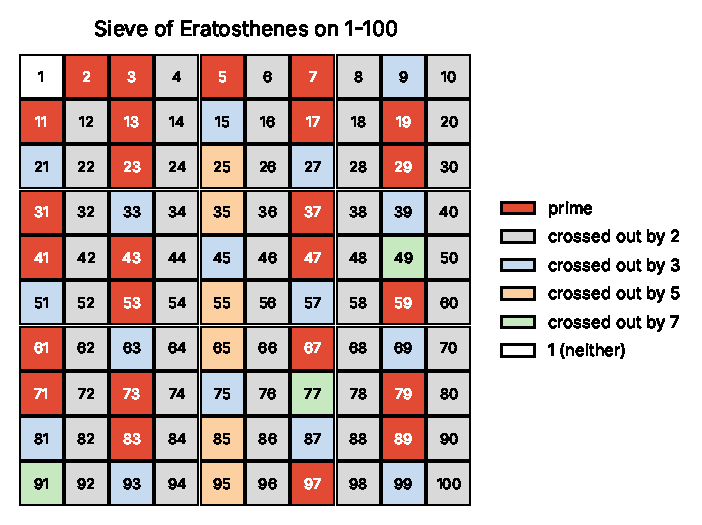
\includegraphics[width=0.85\linewidth]{figs/primes_sieve.pdf}
\caption{The sieve of Eratosthenes on $1$--$100$. Primes are shown in red. Every composite number is colored by its smallest prime factor, which is the prime whose pass of the sieve first crosses it out. Because $\sqrt{100}=10$, the passes for $2,3,5,7$ already remove every composite, in agreement with Lemma~2.}
\label{fig:primes-sieve}
\end{figure}

\begin{sample}{Sieving up to 50}
List the primes up to $x=50$ with the sieve and count them.

\textbf{Step 1: decide when to stop.} We need passes only for primes $p$ with $p^2\le50$, namely $2,3,5,7$ (since $7^2=49\le50<121=11^2$).

\textbf{Step 2: pass for 2.} Cross out $4,6,8,\dots,50$.

\textbf{Step 3: pass for 3.} Cross out $9,12,15,\dots,48$ (many already gone).

\textbf{Step 4: pass for 5.} Cross out $25,30,35,40,45,50$.

\textbf{Step 5: pass for 7.} Cross out $49$ (the only multiple of 7 that is at least $49$ and at most $50$).

\textbf{Step 6: read off the survivors.} $2,3,5,7,11,13,17,19,23,29,31,37,41,43,47$.
\[
\boxed{\text{15 primes up to 50.}}
\]
\end{sample}

\begin{pycode}
import numpy as np

def sieve(x):
    """Return a numpy array of all primes <= x."""
    is_prime = np.ones(x + 1, dtype=bool)   # start: everything unmarked
    is_prime[:2] = False                    # 0 and 1 are not prime
    p = 2
    while p * p <= x:
        if is_prime[p]:                     # p survived, so p is prime
            is_prime[p*p::p] = False        # cross out p^2, p^2+p, ...
        p += 1
    return np.nonzero(is_prime)[0]          # indices still marked True

primes = sieve(100)
print(len(primes), primes[-1])              # prints: 25 97
\end{pycode}

The slice \texttt{is\_prime[p*p::p]} means ``every $p$-th entry, starting at index $p^2$'', which is exactly step 3. The same job is done by \texttt{qmnt.primes\_upto(x)}.

How much work is the sieve? The pass for $p$ crosses out about $x/p$ numbers, so the total is about $x\sum_{p\le\sqrt x}1/p$. A theorem of Mertens, which we do not prove (see \cite{hardywright}, Chapter~22), says $\sum_{p\le y}1/p$ grows like $\log\log y$, extraordinarily slowly. So in practice the sieve costs only a little more than writing the list down. Listing the first $10^6$ integers' primes takes a fraction of a second.

\begin{checkpoint}
When sieving up to 200, which is the last prime whose multiples you must cross out?
\end{checkpoint}
\checkanswer{$13$: since $13^2=169\le200$ but the next prime has $17^2=289>200$.}

\begin{keyideas}
\item The sieve lists all primes up to $x$ by crossing out multiples of each surviving $p$, starting at $p^2$, for $p\le\sqrt x$.
\item It is correct because every composite $n\le x$ has a smallest prime factor $p$ with $p^2\le n$.
\item Its cost grows only slightly faster than $x$.
\end{keyideas}

%=====================================================================
\section{Counting primes: the function $\pi(x)$}\label{sec:primes-pi}

\begin{quote}
\textbf{Definition.} For a real number $x$, the \emph{prime counting function} $\pi(x)$ is the number of primes $p$ with $p\le x$.
\end{quote}

So $\pi(10)=4$ (the primes $2,3,5,7$), $\pi(30)=10$, $\pi(2.5)=1$ and $\pi(1)=0$. As $x$ increases, $\pi(x)$ stays constant until $x$ reaches a prime, where it jumps up by exactly 1. It is a \emph{step function} (\cref{fig:primes-pi-small}).

\begin{pitfall}
In $\pi(x)$ the letter $\pi$ is the name of a function, not the number $3.14159\ldots$ Context always decides; in this chapter, $\pi(x)$ with an argument means the prime counting function, while the number $\pi$ appears in expressions like $2\pi/\log2$. A second trap: $\pi(n)$ is \emph{how many} primes are at most $n$, while $p_n$ denotes the \emph{$n$-th prime} ($p_1=2$, $p_2=3$, $p_6=13$, $p_{25}=97$). The two are inverse to each other in the sense that $\pi(p_n)=n$.
\end{pitfall}

Counting with the sieve gives \cref{tab:primes-pi}. Look at the last column, the \emph{average spacing} $x/\pi(x)$ between primes up to $x$. Each time $x$ grows by a factor 10, the average spacing grows by about the same amount: the increments are $1.50,\ 1.95,\ 2.18,\ 2.29,\ 2.31$, creeping toward $\log10=2.3026$. That is exactly how a function of the form $\log x$ behaves, since $\log(10x)=\log x+\log 10$. This pattern, that near $x$ primes are spaced by about $\log x$, is what the young Gauss noticed in his own tables around 1792.

\begin{table}[htbp]\centering
\caption{The prime counting function and its approximations. $\mathrm{Li}(x)=\int_2^x\dd t/\log t$ is defined in \cref{eq:primes-Li}. All entries computed by the sieve and by numerical integration (verified in this chapter's check script).}
\label{tab:primes-pi}
\begin{tabular}{rrrrcrr}
\toprule
$x$ & $\pi(x)$ & $x/\log x$ & $\mathrm{Li}(x)$ & $\dfrac{\pi(x)}{x/\log x}$ & $\pi(x)-\mathrm{Li}(x)$ & $x/\pi(x)$\\
\midrule
$10$ & 4 & 4.343 & 5.120 & 0.921 & $-1.12$ & 2.500\\
$10^2$ & 25 & 21.715 & 29.081 & 1.151 & $-4.08$ & 4.000\\
$10^3$ & 168 & 144.765 & 176.564 & 1.161 & $-8.56$ & 5.952\\
$10^4$ & 1229 & 1085.736 & 1245.092 & 1.132 & $-16.09$ & 8.137\\
$10^5$ & 9592 & 8685.890 & 9628.764 & 1.104 & $-36.76$ & 10.425\\
$10^6$ & 78498 & 72382.414 & 78626.504 & 1.084 & $-128.50$ & 12.739\\
\bottomrule
\end{tabular}
\end{table}

\begin{figure}[htbp]\centering
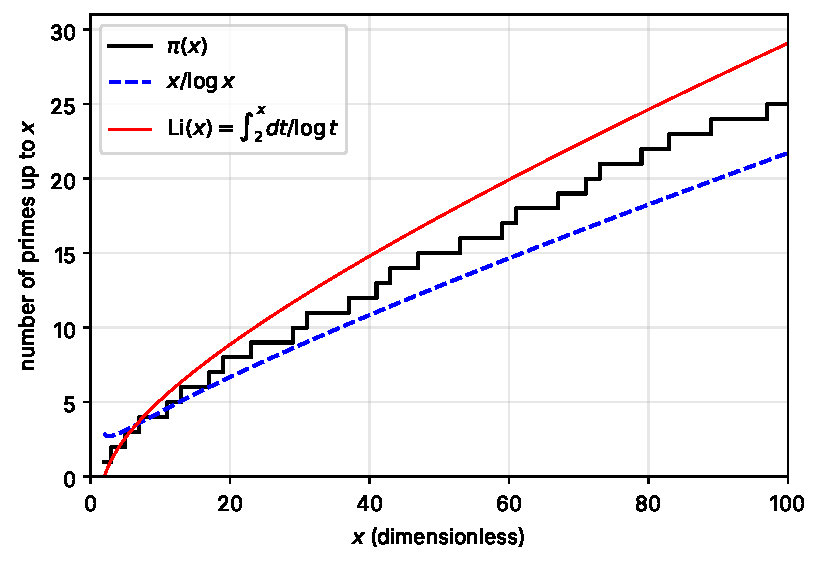
\includegraphics[width=0.85\linewidth]{figs/primes_pi_small.pdf}
\caption{The prime counting function $\pi(x)$ (staircase) for $2\le x\le100$, with the two smooth approximations of the prime number theorem: $x/\log x$ (below the staircase over most of this range) and $\mathrm{Li}(x)=\int_2^x\dd t/\log t$ (close to the staircase). At $x=100$ the three values are $25$, $21.7$ and $29.1$.}
\label{fig:primes-pi-small}
\end{figure}

\begin{pycode}
import numpy as np, mpmath, qmnt
primes = qmnt.primes_upto(10**6)
for e in range(1, 7):
    x = 10**e
    pi_x = np.searchsorted(primes, x, side="right")   # number of primes <= x
    Li = float(mpmath.li(x, offset=True))              # integral from 2 to x
    print(x, pi_x, round(x/np.log(x), 3), round(Li, 3), round(x/pi_x, 3))
\end{pycode}

Here \texttt{np.searchsorted(primes, x, side="right")} returns the position at which $x$ would be inserted into the sorted array of primes, which is the number of primes $\le x$. The option \texttt{offset=True} makes \texttt{mpmath.li} integrate from 2 rather than from 0.

\begin{checkpoint}
At which values of $x$ in $[10,20]$ does $\pi(x)$ jump, and what is $\pi(20)$?
\end{checkpoint}
\checkanswer{It jumps by 1 at $x=11,13,17,19$. Since $\pi(10)=4$, we get $\pi(20)=8$.}

\begin{keyideas}
\item $\pi(x)$ counts primes up to $x$; it is a step function with unit jumps at the primes.
\item Numerically, the average spacing $x/\pi(x)$ grows by about $\log10$ per decade (\cref{tab:primes-pi}): primes near $x$ are spaced by roughly $\log x$.
\end{keyideas}

%=====================================================================
\section{The prime number theorem}\label{sec:primes-pnt}

\subsection{Statement}

Recall from Chapter~\ref{ch:asymptotics} that $f(x)\sim g(x)$ (``$f$ is asymptotic to $g$'') means $f(x)/g(x)\to1$ as $x\to\infty$.

\begin{quote}
\textbf{Prime number theorem (PNT).}
\begin{equation}
\pi(x)\sim\frac{x}{\log x}\qquad(x\to\infty).
\label{eq:primes-pnt}
\end{equation}
\end{quote}

\begin{beyond}
\textbf{Status: proved, proof beyond this book.} The PNT was proved in 1896, independently, by Jacques Hadamard and Charles de la Vall\'ee Poussin. Both proofs use the zeta function of Chapter~\ref{ch:zeta} as a function of a complex variable, and the key input is that $\zeta(s)$ has no zeros on the line $\Re s=1$. An ``elementary'' proof (no complex analysis, but not simpler) was found by Erd\H{o}s and Selberg in 1949. Readable accounts: \cite{apostol}, Chapter~13; \cite{davenport}, Chapters~13 and 18; \cite{edwards}, Chapter~5.
\end{beyond}

\subsection{History in brief}

The theorem was conjectured long before it was proved. Gauss, as a teenager around 1792, counted primes in blocks of 1000 and concluded that their density near $x$ is about $1/\log x$; he described this in a letter of 1849. Legendre published in 1798 (refined 1808) the empirical formula $x/(\log x-1.08366)$. Around 1850 Chebyshev proved that the ratio $\pi(x)/(x/\log x)$ is trapped, for all large $x$, between two constants close to 1 (about $0.921$ and $1.106$), and that \emph{if} the ratio has a limit, the limit is 1; \cref{sec:primes-chebyshev} reproduces the spirit of his argument. In 1859 Riemann's eight-page paper \cite{riemann1859} showed that the fine structure of $\pi(x)$ is governed by the zeros of the zeta function. That paper is where the Riemann hypothesis was first stated.

\subsection{The logarithmic integral}

Gauss's density idea suggests a better approximation than $x/\log x$. If a number near $t$ is prime ``with probability'' about $1/\log t$, then the expected number of primes in a short interval $[t,t+\dd t]$ is $\dd t/\log t$, and adding up these contributions gives the \emph{logarithmic integral}
\begin{equation}
\mathrm{Li}(x) = \int_2^x\frac{\dd t}{\log t}.
\label{eq:primes-Li}
\end{equation}
(The ``probability'' language is a heuristic: primes are not random. It is a useful bookkeeping device, not a theorem.)

\begin{pitfall}
Many tables use instead $\mathrm{li}(x)=\int_0^x\dd t/\log t$, where the singularity at $t=1$ is handled by a symmetric limit. The two differ by a constant: $\mathrm{li}(x)=\mathrm{Li}(x)+\mathrm{li}(2)$ with $\mathrm{li}(2)\approx1.045$. For large $x$ the constant is irrelevant; for small $x$ make sure you know which one a table means. This book uses $\mathrm{Li}$.
\end{pitfall}

\textbf{$\mathrm{Li}(x)\sim x/\log x$ (proved).} We show that the two approximations agree to leading order, so \cref{eq:primes-pnt} may equally be written $\pi(x)\sim\mathrm{Li}(x)$.

\emph{Step 1: integrate by parts.} In \cref{eq:primes-Li} take $u=1/\log t$ and $\dd v=\dd t$, so that $\dd u=-\dd t/(t\log^2t)$ and $v=t$:
\begin{align}
\mathrm{Li}(x) &= \Bigl[\frac{t}{\log t}\Bigr]_2^x - \int_2^x t\cdot\Bigl(-\frac{1}{t\log^2t}\Bigr)\dd t \notag\\
&= \frac{x}{\log x}-\frac{2}{\log2}+\int_2^x\frac{\dd t}{\log^2t}.
\label{eq:primes-Liparts}
\end{align}

\emph{Step 2: bound the leftover integral.} Split it at $\sqrt x$ (assume $x>4$ so that $\sqrt x>2$). On $[2,\sqrt x]$ the integrand is at most $1/\log^22$ and the interval has length less than $\sqrt x$. On $[\sqrt x,x]$ the integrand is at most $1/\log^2\sqrt x=4/\log^2x$ and the interval has length less than $x$. So
\[
0<\int_2^x\frac{\dd t}{\log^2t} < \frac{\sqrt x}{\log^22}+\frac{4x}{\log^2x}.
\]

\emph{Step 3: compare with $x/\log x$.} Divide the bound by $x/\log x$:
\[
\frac{\sqrt x}{\log^22}\cdot\frac{\log x}{x}+\frac{4x}{\log^2x}\cdot\frac{\log x}{x}=\frac{\log x}{\sqrt x\,\log^22}+\frac{4}{\log x}\longrightarrow0 .
\]
(The first term tends to zero because $\log x$ grows more slowly than any positive power of $x$, Chapter~\ref{ch:asymptotics}.) Also $(2/\log2)/(x/\log x)\to0$. Dividing \cref{eq:primes-Liparts} by $x/\log x$ therefore gives $\mathrm{Li}(x)/(x/\log x)\to1$. $\blacksquare$

Step 3 also tells us \emph{how fast} the ratio approaches 1: the correction is of relative size $1/\log x$, which shrinks painfully slowly. At $x=10^6$, $1/\log x\approx0.072$, matching the $8\%$ excess of $\pi(x)$ over $x/\log x$ in \cref{tab:primes-pi}. Repeating the integration by parts (Problem~25) gives the \emph{asymptotic series}
\[
\mathrm{Li}(x)=\frac{x}{\log x}+\frac{x}{\log^2x}+\frac{2x}{\log^3x}+\dots,
\]
whose first terms improve the approximation, although (like Stirling's series in Chapter~\ref{ch:asymptotics}) the full series does not converge.

\begin{figure}[htbp]\centering
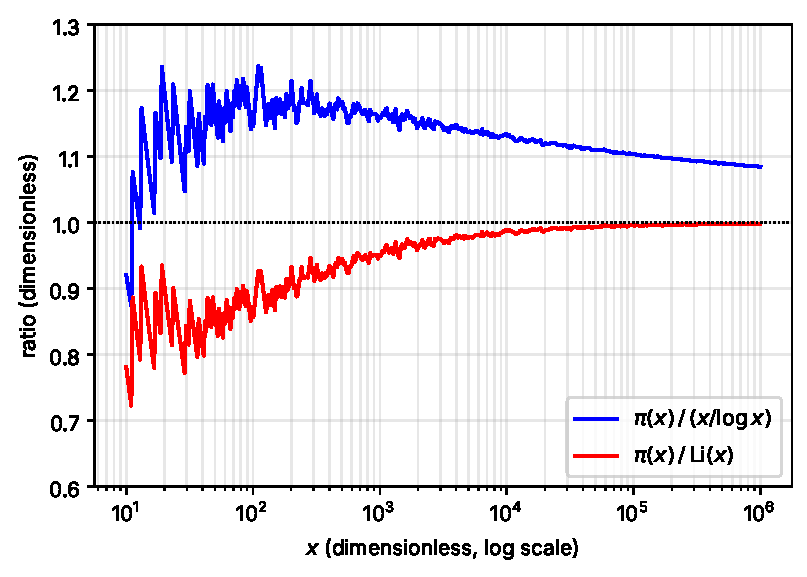
\includegraphics[width=0.85\linewidth]{figs/primes_ratio.pdf}
\caption{Ratios $\pi(x)/(x/\log x)$ and $\pi(x)/\mathrm{Li}(x)$ for $10\le x\le10^6$ (logarithmic $x$-axis). Both tend to 1, as the prime number theorem requires, but $\pi(x)/\mathrm{Li}(x)$ is within a fraction of a percent of 1 over most of the range while $\pi(x)/(x/\log x)$ is still about $1.08$ at $x=10^6$.}
\label{fig:primes-ratio}
\end{figure}

\begin{sample}{How good are the two approximations?}
Using \cref{tab:primes-pi}, compute the relative errors of $x/\log x$ and $\mathrm{Li}(x)$ as approximations to $\pi(x)$ at $x=10^3$ and $x=10^6$. Then test the density picture on the interval $[10^4,10^5]$.

\textbf{Step 1: $x=10^3$.} Relative error of $x/\log x$: $(144.765-168)/168=-0.138$. Relative error of $\mathrm{Li}$: $(176.564-168)/168=+0.051$.

\textbf{Step 2: $x=10^6$.} $(72382.414-78498)/78498=-0.078$ and $(78626.504-78498)/78498=+0.0016$.

\textbf{Step 3: an interval.} The density picture predicts that the number of primes in $(10^4,10^5]$ is about $\int_{10^4}^{10^5}\dd t/\log t=\mathrm{Li}(10^5)-\mathrm{Li}(10^4)=9628.764-1245.092=8383.67$. The true count is $\pi(10^5)-\pi(10^4)=9592-1229=8363$.
\[
\boxed{\begin{array}{l}
x/\log x:\ -13.8\%\ (10^3),\ -7.8\%\ (10^6);\quad \mathrm{Li}:\ +5.1\%\ (10^3),\ +0.16\%\ (10^6)\\
\text{primes in }(10^4,10^5]:\ 8363\ \text{actual vs } 8383.7\ \text{predicted}
\end{array}}
\]
Both approximations are asymptotically correct, but $\mathrm{Li}$ is far better at every height we can check.
\end{sample}

\subsection{Mean spacing of primes}

If primes near $x$ have density $1/\log x$, their \emph{local mean spacing} is the reciprocal, $\log x$. At $x=10^6$ that is $\log10^6=13.82$. The average spacing over the \emph{whole} range up to $10^6$ is smaller, $10^6/78498=12.74$, because it includes the crowded small primes. Compare Chapter~\ref{ch:counting-zeros}, where the Riemann zeros get a local mean spacing $\gap_n$ in exactly the same way, as the reciprocal of a smooth density.

\subsection{The error term and the Riemann hypothesis}

How large is $\pi(x)-\mathrm{Li}(x)$? In \cref{tab:primes-pi} it is negative and grows in size, but slowly compared with $\pi(x)$ itself.

\begin{beyond}
\textbf{What is known.} De la Vall\'ee Poussin proved $\pi(x)=\mathrm{Li}(x)+\order\bigl(x\,e^{-c\sqrt{\log x}}\bigr)$ for some constant $c>0$, an error smaller than $x/\log^kx$ for every $k$ (proof: \cite{davenport}, Chapter~18).

\textbf{The Riemann hypothesis connection.} It is a theorem (von Koch, 1901) that the Riemann hypothesis of Chapter~\ref{ch:zeta} is \emph{equivalent} to the statement $\pi(x)=\mathrm{Li}(x)+\order(\sqrt x\log x)$. The Riemann hypothesis itself is \textbf{open}: it has been neither proved nor disproved. So the best possible error term for counting primes is an open problem, and it is controlled by the zeros (\cite{edwards}, Chapter~5).

\textbf{A warning about numerical evidence.} In every case ever computed directly, $\pi(x)<\mathrm{Li}(x)$. Yet Littlewood proved in 1914 that $\pi(x)-\mathrm{Li}(x)$ changes sign infinitely often. The first sign change is known to occur only at astronomically large $x$. Tables, however large, can mislead.
\end{beyond}

\begin{checkpoint}
``Since $\pi(x)\sim x/\log x$, the difference $\pi(x)-x/\log x$ tends to zero.'' True or false?
\end{checkpoint}
\checkanswer{False. $\sim$ says the \emph{ratio} tends to 1. The difference grows without bound: it is $6115.6$ at $x=10^6$ (from \cref{tab:primes-pi}) and is of order $x/\log^2x$.}

\begin{keyideas}
\item PNT: $\pi(x)\sim x/\log x\sim\mathrm{Li}(x)$ (\cref{eq:primes-pnt,eq:primes-Li}); proved in 1896, proof beyond this book.
\item $\mathrm{Li}(x)\sim x/\log x$ is proved here by integration by parts (\cref{eq:primes-Liparts}); the relative difference is of order $1/\log x$.
\item Near $x$ the primes have density $1/\log x$ and mean spacing $\log x$ (heuristic picture, consistent with the PNT).
\item The size of $\pi(x)-\mathrm{Li}(x)$ is governed by the zeta zeros; the Riemann hypothesis, which would make it $\order(\sqrt x\log x)$, is open.
\end{keyideas}

%=====================================================================
\section{A proven bound: Chebyshev's argument}\label{sec:primes-chebyshev}

The PNT is beyond us, but a weaker statement of the right shape is not. It introduces a function that appears throughout the rest of the chapter.

\begin{quote}
\textbf{Definition.} Chebyshev's \emph{theta function} is
\begin{equation}
\theta(x)=\sum_{p\le x}\log p ,
\label{eq:primes-theta}
\end{equation}
the sum of the logarithms of all primes up to $x$. Equivalently $\theta(x)=\log\bigl(\prod_{p\le x}p\bigr)$.
\end{quote}

So $\theta(10)=\log(2\cdot3\cdot5\cdot7)=\log210$. Where $\pi(x)$ counts each prime with weight 1, $\theta(x)$ counts it with weight $\log p$, its ``size''.

\textbf{Theorem (proved).} \emph{For every integer $n\ge1$,}
\begin{equation}
\theta(2n)-\theta(n) < n\log4,
\label{eq:primes-cheb1}
\end{equation}
\emph{and for every real $x\ge1$, $\theta(x)<(4\log2)\,x\approx2.77\,x$.}

\emph{Proof of \cref{eq:primes-cheb1}.} Recall the binomial coefficient $\binom{2n}{n}=\frac{(2n)!}{n!\,n!}$, the number of ways of choosing $n$ objects from $2n$, which is a positive integer.
\begin{enumerate}
\item \emph{Every prime $p$ with $n<p\le2n$ divides $\binom{2n}{n}$.} Such a $p$ is one of the factors of $(2n)!=1\cdot2\cdots(2n)$, so $p\mid(2n)!=\binom{2n}{n}\,(n!)^2$. By Euclid's lemma $p$ divides $\binom{2n}{n}$ or $(n!)^2$. It cannot divide $(n!)^2=(1\cdot2\cdots n)^2$: by the repeated Euclid's lemma it would then divide one of the factors $1,\dots,n$, all of which are positive and smaller than $p$. So $p\mid\binom{2n}{n}$.
\item \emph{Their product divides $\binom{2n}{n}$.} Each such prime appears in the factorization of $\binom{2n}{n}$ (by uniqueness), and they are distinct, so their product $\prod_{n<p\le2n}p$ divides $\binom{2n}{n}$, and therefore $\prod_{n<p\le2n}p\le\binom{2n}{n}$.
\item \emph{$\binom{2n}{n}<4^n$.} By the binomial expansion, $4^n=(1+1)^{2n}=\sum_{k=0}^{2n}\binom{2n}{k}$, a sum of positive terms of which $\binom{2n}{n}$ is one, and for $n\ge1$ there are other terms (e.g.\ $\binom{2n}{0}=1$).
\item \emph{Take logs.} $\theta(2n)-\theta(n)=\sum_{n<p\le2n}\log p=\log\prod_{n<p\le2n}p\le\log\binom{2n}{n}<n\log4$.
\end{enumerate}

\emph{Proof of $\theta(x)<(4\log2)x$.} Given $x\ge1$, choose the integer $k\ge1$ with $2^{k-1}\le x<2^k$. Since $\theta$ never decreases and $\theta(1)=0$, a telescoping sum (Chapter~\ref{ch:series}) gives
\begin{align*}
\theta(x)\le\theta(2^k) &= \sum_{j=1}^{k}\bigl[\theta(2^j)-\theta(2^{j-1})\bigr] \\
&< \sum_{j=1}^{k}2^{j-1}\log4 \quad\text{(\cref{eq:primes-cheb1} with $n=2^{j-1}$)}\\
&= (2^k-1)\log4 \quad\text{(geometric series)}\\
&< 2^k\log4 \le 2x\log4=(4\log2)\,x \quad\text{(since $2^{k-1}\le x$)}. \qquad\blacksquare
\end{align*}

\textbf{Corollary (proved): $\pi(x)=\order(x/\log x)$.} For $x>1$, the primes in $(\sqrt x,x]$ each contribute more than $\log\sqrt x=\tfrac12\log x$ to $\theta(x)$, so
\[
\theta(x)\ \ge \sum_{\sqrt x<p\le x}\log p\ \ge\ \bigl[\pi(x)-\pi(\sqrt x)\bigr]\tfrac12\log x .
\]
Rearranging and using $\pi(\sqrt x)\le\sqrt x$ and $\theta(x)<(4\log2)x$,
\begin{equation}
\pi(x)\ \le\ \pi(\sqrt x)+\frac{2\,\theta(x)}{\log x}\ <\ \sqrt x+(8\log2)\frac{x}{\log x}.
\label{eq:primes-chebbound}
\end{equation}
The constant $8\log2\approx5.55$ is generous (at $x=10^6$ the bound is about $402{,}000$ against the true $78{,}498$), but the \emph{shape} $x/\log x$ is exactly the one in the PNT, and the argument used nothing but factorization. Chebyshev's sharper version of this reasoning gave the constants $0.921$ and $1.106$ quoted above; Problem~23 proves a lower bound of the same shape.

\begin{sample}{Chebyshev's divisibility for $n=10$}
Check each step of the proof of \cref{eq:primes-cheb1} for $n=10$.

\textbf{Step 1: the primes in $(10,20]$.} They are $11,13,17,19$, with product $11\cdot13\cdot17\cdot19=46189$.

\textbf{Step 2: the binomial coefficient.} $\binom{20}{10}=184756$.

\textbf{Step 3: divisibility.} $184756/46189=4$ exactly, so $184756=2^2\cdot11\cdot13\cdot17\cdot19$; the product of the four primes divides it, as claimed.

\textbf{Step 4: the bound.} $\theta(20)-\theta(10)=\log46189=10.7405$, while $10\log4=13.8629$.
\[
\boxed{\theta(20)-\theta(10)=\log 46189\approx10.74<10\log4\approx13.86.}
\]
\end{sample}

\begin{keyideas}
\item $\theta(x)=\sum_{p\le x}\log p$ weights each prime by its logarithm (\cref{eq:primes-theta}).
\item Using only unique factorization and the binomial coefficient $\binom{2n}{n}<4^n$, one proves $\theta(x)<(4\log2)x$ and $\pi(x)<\sqrt x+(8\log2)x/\log x$ (\cref{eq:primes-cheb1,eq:primes-chebbound}): primes thin out at the rate the PNT predicts, up to a constant.
\end{keyideas}

%=====================================================================
\section{Prime powers and the von Mangoldt function}\label{sec:primes-mangoldt}

\subsection{Prime powers}

A \emph{prime power} is a number of the form $q=p^m$ with $p$ prime and $m\ge1$ an integer. Primes themselves are prime powers with $m=1$. The prime powers up to 30 are
\[
2,3,4,5,7,8,9,11,13,16,17,19,23,25,27,29 ,
\]
where $4=2^2$, $8=2^3$, $9=3^2$, $16=2^4$, $25=5^2$ and $27=3^3$ are the ones that are not prime. By unique factorization, a prime power determines its $p$ and $m$: $q=p^m$ has exactly one prime factor.

Why single out prime powers? The paper's Eq.~(4) contains the waves $\sin(mt\log p)$, and $m\log p=\log(p^m)$, so its frequencies are precisely the logarithms of prime powers. The next definition gives each prime power its natural weight.

\subsection{The von Mangoldt function}

\begin{quote}
\textbf{Definition.} The \emph{von Mangoldt function} is defined for positive integers $k$ by
\begin{equation}
\Lambda(k)=\begin{cases}\log p, & \text{if } k=p^m \text{ for a prime } p \text{ and an integer } m\ge1,\\[2pt] 0, & \text{otherwise.}\end{cases}
\label{eq:primes-Lambda}
\end{equation}
\end{quote}

So $\Lambda$ is zero except at prime powers, and at a power of $p$ it equals $\log p$, whatever the exponent. \Cref{tab:primes-Lambda} lists the first values and \cref{fig:primes-mangoldt} plots them.

\begin{table}[htbp]\centering
\caption{The von Mangoldt function for $k=1,\dots,12$.}
\label{tab:primes-Lambda}
\begin{tabular}{lcccccccccccc}
\toprule
$k$ & 1 & 2 & 3 & 4 & 5 & 6 & 7 & 8 & 9 & 10 & 11 & 12\\
\midrule
$\Lambda(k)$ & 0 & $\log2$ & $\log3$ & $\log2$ & $\log5$ & 0 & $\log7$ & $\log2$ & $\log3$ & 0 & $\log11$ & 0\\
value & 0 & 0.693 & 1.099 & 0.693 & 1.609 & 0 & 1.946 & 0.693 & 1.099 & 0 & 2.398 & 0\\
\bottomrule
\end{tabular}
\end{table}

\begin{figure}[htbp]\centering
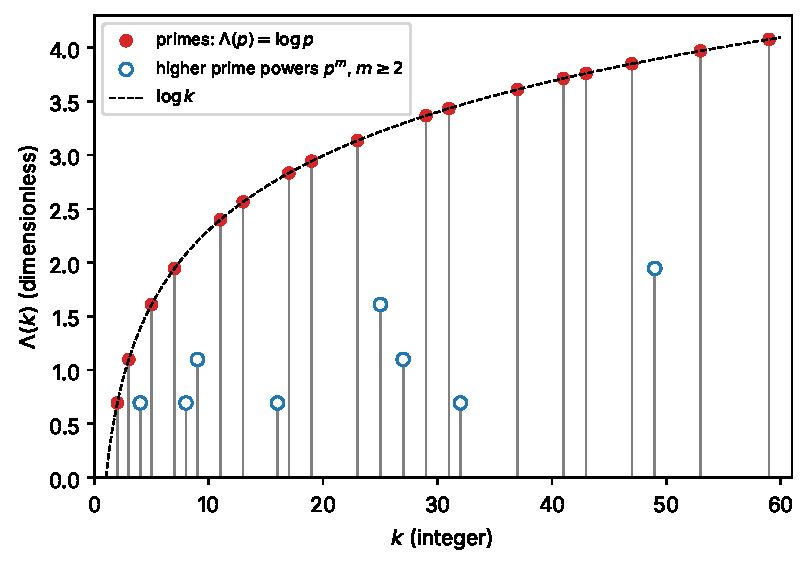
\includegraphics[width=0.85\linewidth]{figs/primes_mangoldt.pdf}
\caption{The von Mangoldt function $\Lambda(k)$ for $1\le k\le60$. Primes (filled markers) sit on the curve $\log k$ (dashed); higher prime powers such as $4,8,16,32$ (open markers) sit lower, at the height $\log p$ of their prime. At all other integers $\Lambda(k)=0$.}
\label{fig:primes-mangoldt}
\end{figure}

\begin{pitfall}
$\Lambda(1)=0$: the number $1=p^0$ is \emph{not} counted as a prime power, because the definition requires $m\ge1$. And $\Lambda(8)=\log2$, not $\log8$: the weight is the log of the underlying prime.
\end{pitfall}

\subsection{The key identity}

The weights in \cref{eq:primes-Lambda} look odd until you see what they add up to.

\textbf{Theorem (proved).} \emph{For every positive integer $n$,}
\begin{equation}
\sum_{d\mid n}\Lambda(d)=\log n ,
\label{eq:primes-divsum}
\end{equation}
\emph{where the sum runs over all positive divisors $d$ of $n$.}

\emph{Proof.} For $n=1$ the only divisor is $1$ and both sides are 0. For $n\ge2$ write the canonical factorization $n=p_1^{a_1}\cdots p_k^{a_k}$. Only divisors that are prime powers contribute to the sum. A prime power $p^j$ divides $n$ exactly when $p$ is one of the $p_i$ and $1\le j\le a_i$ (by uniqueness of factorization, the prime powers dividing $n$ are of this form, and each of these does divide $n$). For each $i$ there are $a_i$ such divisors $p_i^1,\dots,p_i^{a_i}$, each contributing $\log p_i$. Therefore
\[
\sum_{d\mid n}\Lambda(d)=\sum_{i=1}^{k}a_i\log p_i=\log n,
\]
where the last step is \cref{eq:primes-logfta}. $\blacksquare$

In words: $\Lambda$ is the weighting that makes the prime-power divisors of $n$ add up exactly to the size $\log n$ of $n$. It is ``the logarithm, broken into its prime pieces''. This is why $\Lambda$ appears in the logarithmic derivative of the zeta function (Chapter~\ref{ch:explicit-formula}).

\begin{sample}{Checking the identity for $n=12$}
Verify \cref{eq:primes-divsum} for $n=12$.

\textbf{Step 1: list the divisors.} $1,2,3,4,6,12$.

\textbf{Step 2: their $\Lambda$ values} (from \cref{tab:primes-Lambda}): $0,\ \log2,\ \log3,\ \log2,\ 0,\ 0$.

\textbf{Step 3: add.} $\log2+\log3+\log2=\log(2\cdot3\cdot2)=\log12$.

\textbf{Step 4: numerical value.}
\[
\boxed{\sum_{d\mid12}\Lambda(d)=2\log2+\log3=\log12\approx2.4849.}
\]
\end{sample}

\begin{keyideas}
\item A prime power is $q=p^m$, $m\ge1$; the frequencies $m\log p$ of the paper are the numbers $\log q$.
\item $\Lambda(q)=\log p$ at $q=p^m$ and $0$ elsewhere (\cref{eq:primes-Lambda}); $\Lambda(1)=0$.
\item $\sum_{d\mid n}\Lambda(d)=\log n$ (\cref{eq:primes-divsum}): $\Lambda$ splits $\log n$ into prime-power pieces.
\end{keyideas}

%=====================================================================
\section{Chebyshev's function $\psi(x)$}\label{sec:primes-psi}

\begin{quote}
\textbf{Definition.} Chebyshev's \emph{psi function} is
\begin{equation}
\psi(x)=\sum_{k\le x}\Lambda(k)=\sum_{p^m\le x}\log p ,
\label{eq:primes-psi}
\end{equation}
the sum over all prime powers $p^m\le x$ (with $m\ge1$) of $\log p$.
\end{quote}

Like $\pi(x)$, $\psi(x)$ is a step function, but its steps sit at all prime powers and have height $\log p$ (\cref{fig:primes-psi}a).

\subsection{Three properties}

\textbf{(a) $\psi$ is built from $\theta$.} Group the terms of \cref{eq:primes-psi} by the exponent $m$. The prime powers $p^m\le x$ with a fixed $m$ are exactly those with $p\le x^{1/m}$, and they contribute $\sum_{p\le x^{1/m}}\log p=\theta(x^{1/m})$. So
\begin{equation}
\psi(x)=\theta(x)+\theta(x^{1/2})+\theta(x^{1/3})+\dots
\label{eq:primes-psitheta}
\end{equation}
The sum is finite: once $m>\log x/\log2$ we have $x^{1/m}<2$ and $\theta(x^{1/m})=0$. The $m=1$ term dominates; the others add up to something much smaller (Problem~22 shows the extra amount is $\order(\sqrt x\log^2x)$).

\textbf{(b) $\psi$ is the logarithm of a least common multiple.} For a positive integer $N$, let $\mathrm{lcm}(1,\dots,N)$ be the smallest positive integer divisible by each of $1,2,\dots,N$. Write $\lfloor y\rfloor$ (the \emph{floor} of $y$) for the largest integer not exceeding $y$. A prime $p$ appears in $\mathrm{lcm}(1,\dots,N)$ with exponent equal to the largest $m$ with $p^m\le N$ (that power must be divisible, and no larger power of $p$ is needed), namely $m=\lfloor\log N/\log p\rfloor$. Taking logs,
\[
\log\mathrm{lcm}(1,\dots,N)=\sum_{p\le N}\Bigl\lfloor\frac{\log N}{\log p}\Bigr\rfloor\log p .
\]
On the other hand, in \cref{eq:primes-psi} each prime $p\le N$ contributes $\log p$ once for each $m\ge1$ with $p^m\le N$, that is $\lfloor\log N/\log p\rfloor$ times. The two expressions agree:
\begin{equation}
\psi(N)=\log\mathrm{lcm}(1,2,\dots,N).
\label{eq:primes-lcm}
\end{equation}

\textbf{(c) $\psi(x)\le\pi(x)\log x$.} From the counting in (b), each prime $p\le x$ contributes $\lfloor\log x/\log p\rfloor\log p\le(\log x/\log p)\log p=\log x$. There are $\pi(x)$ such primes, so
\begin{equation}
\psi(x)\le\pi(x)\log x .
\label{eq:primes-psipi}
\end{equation}

\subsection{The PNT in Chebyshev's form}

\begin{beyond}
\textbf{Proved, proof beyond this book.} The statements $\pi(x)\sim x/\log x$, $\theta(x)\sim x$ and $\psi(x)\sim x$ are equivalent: any one implies the others. One direction is suggested by \cref{eq:primes-psipi}; the full argument uses a summation-by-parts technique (\cite{apostol}, Theorem~4.4). So the PNT can be stated as
\begin{equation}
\psi(x)\sim x .
\label{eq:primes-psix}
\end{equation}
This is the most natural form of the PNT: the prime powers, each weighted by $\log p$, accumulate at an average rate of exactly 1 per unit of $x$.
\end{beyond}

\Cref{tab:primes-psi} shows how quickly $\psi(x)/x$ approaches 1, much faster than $\pi(x)/(x/\log x)$ did in \cref{tab:primes-pi}. Panel (b) of \cref{fig:primes-psi} shows that $\psi(x)-x$ wanders on the scale of $\sqrt x$.

\begin{table}[htbp]\centering
\caption{Chebyshev's function $\psi(x)$ compared with $x$ (computed in the check script).}
\label{tab:primes-psi}
\begin{tabular}{rrrr}
\toprule
$x$ & $\psi(x)$ & $\psi(x)/x$ & $\psi(x)-x$\\
\midrule
$10$ & 7.832 & 0.783 & $-2.168$\\
$10^2$ & 94.045 & 0.940 & $-5.955$\\
$10^3$ & 996.681 & 0.997 & $-3.319$\\
$10^4$ & 10013.391 & 1.001 & $+13.391$\\
\bottomrule
\end{tabular}
\end{table}

\begin{figure}[htbp]\centering
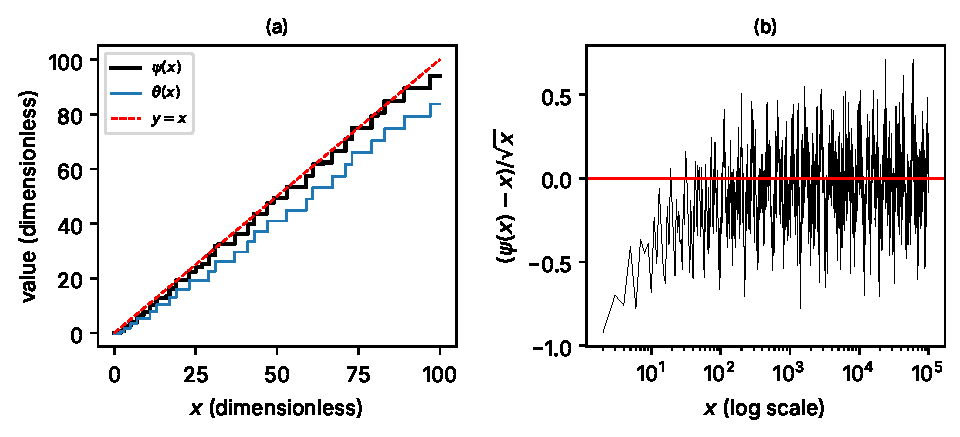
\includegraphics[width=\linewidth]{figs/primes_psi.pdf}
\caption{(a) Chebyshev's functions $\psi(x)$ (steps at every prime power) and $\theta(x)$ (steps at primes only) for $x\le100$, with the line $y=x$ that the PNT says $\psi$ follows. (b) The scaled difference $(\psi(x)-x)/\sqrt x$ at integers $x$ up to $10^5$: the deviation of $\psi(x)$ from $x$ fluctuates on the scale $\sqrt x$, the scale tied to the critical line $\Re s=\tfrac12$ of the zeta function.}
\label{fig:primes-psi}
\end{figure}

\begin{sample}{$\psi(10)$ and $\psi(30)$ as least common multiples}
Compute $\psi(10)$ and $\psi(30)$ using \cref{eq:primes-lcm}.

\textbf{Step 1: $\mathrm{lcm}(1,\dots,10)$.} The largest powers of each prime not exceeding 10 are $2^3=8$, $3^2=9$, $5$, $7$. So $\mathrm{lcm}=8\cdot9\cdot5\cdot7=2520$ and $\psi(10)=\log2520=7.8320$. Check with \cref{eq:primes-psi}: the prime powers up to 10 are $2,3,4,5,7,8,9$, contributing $\log2+\log3+\log2+\log5+\log7+\log2+\log3=\log(2^3\cdot3^2\cdot5\cdot7)$, the same.

\textbf{Step 2: $\mathrm{lcm}(1,\dots,30)$.} Largest prime powers up to 30: $2^4=16$, $3^3=27$, $5^2=25$, and the primes $7,11,13,17,19,23,29$.

\textbf{Step 3: add logarithms.}
\[
\psi(30)=4\log2+3\log3+2\log5+\log7+\log11+\log13+\log17+\log19+\log23+\log29 .
\]
Numerically: $2.7726+3.2958+3.2189+1.9459+2.3979+2.5649+2.8332+2.9444+3.1355+3.3673=28.4765$.

\textbf{Step 4: compare with $x$.}
\[
\boxed{\psi(10)=\log2520\approx7.832,\qquad\psi(30)\approx28.48,\qquad \psi(30)/30\approx0.949.}
\]
\end{sample}

\begin{pycode}
import numpy as np, qmnt
x = 10000
Lam = np.zeros(x + 1)                 # Lam[k] will hold Lambda(k)
for p in qmnt.primes_upto(x):
    q = int(p)
    while q <= x:                     # q runs over p, p^2, p^3, ...
        Lam[q] = np.log(p)
        q = q * int(p)
psi = np.cumsum(Lam)                  # psi[k] = Lambda(1) + ... + Lambda(k)
print(psi[10], np.log(2520))          # both 7.832...
print(psi[1000], psi[10000] / 10000)  # 996.68..., 1.0013...
\end{pycode}

\begin{beyond}
\textbf{A preview: $\psi(x)$ and the zeros.} Riemann's ideas, made rigorous by von Mangoldt in 1895, give an exact formula: for $x>1$ not a prime power,
\[
\psi(x)=x-\sum_{\rho}\frac{x^{\rho}}{\rho}-\log(2\pi)-\tfrac12\log\bigl(1-x^{-2}\bigr),
\]
where $\rho$ runs over the nontrivial zeros of the zeta function, summed in pairs $\rho,\bar\rho$ in order of increasing $\abs{\Im\rho}$ (proof: \cite{davenport}, Chapter~17; \cite{edwards}, Chapter~3). Each zero $\rho_n=\tfrac12+it_n$ contributes a wave $x^{1/2}e^{it_n\log x}$ in the variable $\log x$, of size $\sqrt x$: the zeros are frequencies of the primes. Chapter~\ref{ch:explicit-formula} turns this duality around, making the prime powers the frequencies of the zeros, which is the content of the paper's Eq.~(4).
\end{beyond}

\begin{checkpoint}
What are $\psi(16)-\psi(15)$ and $\psi(18)-\psi(17)$?
\end{checkpoint}
\checkanswer{$\psi(16)-\psi(15)=\Lambda(16)=\log2\approx0.693$ since $16=2^4$; $\psi(18)-\psi(17)=\Lambda(18)=0$ since $18=2\cdot3^2$ is not a prime power.}

\begin{keyideas}
\item $\psi(x)=\sum_{k\le x}\Lambda(k)$ (\cref{eq:primes-psi}) $=\theta(x)+\theta(x^{1/2})+\dots$ (\cref{eq:primes-psitheta}) $=\log\mathrm{lcm}(1,\dots,\lfloor x\rfloor)$ (\cref{eq:primes-lcm}).
\item $\psi(x)\le\pi(x)\log x$ (proved). PNT in Chebyshev's form: $\psi(x)\sim x$ (equivalence proved, beyond this book).
\item $\psi(x)-x$ fluctuates on the scale $\sqrt x$; the von Mangoldt explicit formula writes it as a sum over the zeta zeros.
\end{keyideas}

%=====================================================================
\section{$\log p$ as the natural size of a prime}\label{sec:primes-logp}

We have now met $\log p$ in five roles. It is worth collecting them, because together they explain why the paper's frequencies are $\log p$ and not $p$.
\begin{enumerate}
\item \emph{Logs turn multiplication into addition.} By \cref{eq:primes-logfta}, every integer is a point $\log n=\sum a_i\log p_i$ built from the ``directions'' $\log2,\log3,\log5,\dots$, and these directions obey no integer relation (\cref{sec:primes-fta}).
\item \emph{Density.} Near $x$, primes have density $1/\log x$ (\cref{sec:primes-pnt}).
\item \emph{Natural weight.} In $\theta$, $\psi$ and $\Lambda$, each prime counts with weight $\log p$, and with these weights the PNT becomes the clean statement $\psi(x)\sim x$, and $\Lambda$ splits $\log n$ exactly (\cref{eq:primes-divsum}).
\item \emph{Digits.} $\log_{10}p=\log p/\log10$ is, up to rounding, the number of decimal digits of $p$: the information needed to write $p$ down.
\item \emph{Frequency.} For real $t$, $p^{-it}=e^{-it\log p}$ (Chapter~\ref{ch:complex}). As $t$ increases, this complex number rotates around the unit circle at angular frequency $\log p$. More generally $(p^m)^{-it}=e^{-imt\log p}$ rotates at $m\log p=\log(p^m)$. So in any expression containing powers $n^{-s}$ with $s=\sigma+it$, each prime power $q$ becomes a wave in $t$ with angular frequency $\log q$ and period
\begin{equation}
P_q=\frac{2\pi}{\log q}.
\label{eq:primes-period}
\end{equation}
\end{enumerate}

\begin{sample}{Periods of the first prime-power waves; the prime-2 wave (RE2)}
Compute the angular frequency $\log q$ and period $P_q=2\pi/\log q$ for $q=2,3,4,5,7,8,9$. Then find the period of the running example RE2, $-\frac1\pi\sum_{m=1}^{3}\frac{\sin(mt\log2)}{m\,2^{m/2}}$.

\textbf{Step 1: logarithms.} $\log2=0.693147$, $\log3=1.098612$, $\log4=1.386294$, $\log5=1.609438$, $\log7=1.945910$, $\log8=2.079442$, $\log9=2.197225$.

\textbf{Step 2: periods} ($2\pi=6.283185$). $P_2=9.0647$, $P_3=5.7192$, $P_4=4.5324$, $P_5=3.9040$, $P_7=3.2289$, $P_8=3.0216$, $P_9=2.8596$.

\textbf{Step 3: the three terms of RE2.} They are the $q=2,4,8$ waves, with periods $P_2$, $P_4=P_2/2$ and $P_8=P_2/3$. Shifting $t$ by $P_2$ changes the argument $mt\log2$ by $mP_2\log2=2\pi m$, a whole number of turns for each $m$, so every term repeats after $P_2$.

\textbf{Step 4: no shorter period.} The $m=1$ term alone has smallest period $P_2$, while the $m=2,3$ terms also repeat after $P_2/2$ and $P_2/3$; a shift that left the sum unchanged would have to leave this slowest component unchanged as well, which first happens at $P_2$.
\[
\boxed{P_2=2\pi/\log2\approx9.065\ \text{(period of RE2)},\quad P_3\approx5.719,\ P_5\approx3.904,\ P_7\approx3.229.}
\]
\end{sample}

Step 4 relied on intuition for the slowest component; Chapter~\ref{ch:fourier-series} makes it precise using orthogonality.

The $q=2$ wave is the slowest and, as we will see next, the strongest. When more primes are included, the waves at $\log3,\log5,\dots$ are incommensurate with it (\cref{sec:primes-fta}), and the sum never repeats.

\subsection{A preview of the zeta connection}

Here is a piece of pure bookkeeping that prepares the paper connection. Consider the double sum over primes $p$ and exponents $m\ge1$ of $p^{-ms}/m$. Each pair $(p,m)$ corresponds to exactly one prime power $n=p^m$, and for that $n$,
\begin{equation}
\frac{\Lambda(n)}{\log n}=\frac{\log p}{\log(p^m)}=\frac{\log p}{m\log p}=\frac1m .
\label{eq:primes-weight}
\end{equation}
So for any $s$ for which the sums converge (Chapter~\ref{ch:series}; $\Re s>1$ suffices),
\begin{equation}
\sum_{p}\sum_{m=1}^{\infty}\frac{p^{-ms}}{m}=\sum_{n=2}^{\infty}\frac{\Lambda(n)}{\log n}\,n^{-s},
\label{eq:primes-logzeta}
\end{equation}
where on the right the terms with $\Lambda(n)=0$ simply vanish. In Chapter~\ref{ch:explicit-formula} you will prove that the left side is $\log\zeta(s)$; here we only note that the right side is a sum over prime powers $n$ with weights $\Lambda(n)/\log n$. On the line $s=\tfrac12+it$ the term $n^{-s}=n^{-1/2}e^{-it\log n}$ is a wave of frequency $\log n$ and amplitude $n^{-1/2}\Lambda(n)/\log n$.

\begin{figure}[htbp]\centering
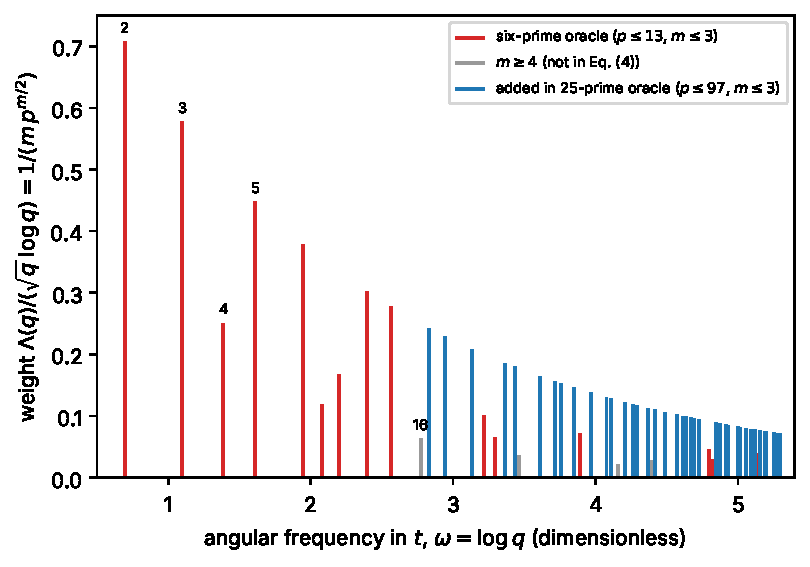
\includegraphics[width=0.85\linewidth]{figs/primes_spectrum.pdf}
\caption{The ``prime-power spectrum'': a vertical line at angular frequency $\omega=\log q$ for every prime power $q\le200$, of height $\Lambda(q)/(\sqrt q\,\log q)=1/(m\,p^{m/2})$ for $q=p^m$. Red: the 18 terms of the six-prime explicit formula ($p\le13$, $m\le3$). Blue: further terms with $m\le3$ and $p\le97$, included in the 25-prime formula. Gray: powers with $m\ge4$ (such as $16$, $32$, $64$, $81$), which Eq.~(4) of the paper omits. The weights decay roughly like $q^{-1/2}$ while the lines crowd together at large $\omega$.}
\label{fig:primes-spectrum}
\end{figure}

\begin{checkpoint}
Which is the larger weight in \cref{fig:primes-spectrum}: that of $q=4=2^2$ or that of $q=13$?
\end{checkpoint}
\checkanswer{$q=4$: $1/(2\cdot2^{1})=0.25$; $q=13$: $1/\sqrt{13}\approx0.277$. So $13$ has the (slightly) larger weight, even though $4$ is the smaller number. The weight depends on both $p$ and $m$.}

\begin{keyideas}
\item $\log p$ is the natural size of a prime: additive coordinate, inverse density, weight in $\theta,\psi,\Lambda$, digit count, and frequency.
\item $p^{-it}=e^{-it\log p}$ rotates at angular frequency $\log p$; prime power $q$ gives period $2\pi/\log q$ (\cref{eq:primes-period}); $2\pi/\log2\approx9.065$.
\item $\Lambda(p^m)/\log(p^m)=1/m$ (\cref{eq:primes-weight}), so double sums over $(p,m)$ are sums over prime powers (\cref{eq:primes-logzeta}).
\end{keyideas}

%=====================================================================
\section{Paper connection}\label{sec:primes-paper}

Everything in the paper's arithmetic side is built from the objects of this chapter. Here is where each appears.

\paragraph{Eq.~(4): a sum over prime powers.} The paper's oracle (Sec.~II~D) is
\[
N_{\rm fl}(t)=-\frac1\pi\sum_{p\in P}\sum_{m=1}^{3}\frac{\sin(mt\log p)}{m\,p^{m/2}},
\]
where $P$ is a finite set of primes. By \cref{eq:primes-weight}, $1/m=\Lambda(p^m)/\log(p^m)$, so with $q=p^m$,
\[
N_{\rm fl}(t)=-\frac1\pi\sum_{\substack{q=p^m,\ p\in P\\ 1\le m\le3}}\frac{\Lambda(q)}{\sqrt q\,\log q}\,\sin(t\log q).
\]
Every term is one line of \cref{fig:primes-spectrum}: a sinusoid in the zero height $t$ with angular frequency $\log q$ and amplitude $\Lambda(q)/(\pi\sqrt q\log q)$. The sine (rather than a cosine) and the factor $-1/\pi$ come from taking an imaginary part of \cref{eq:primes-logzeta} on the critical line; Chapter~\ref{ch:explicit-formula} derives this, and is careful about its formal status. Two things are already visible here. First, the largest amplitude belongs to $q=2$, $m=1$: $1/\sqrt2=0.707$ before the factor $1/\pi$. Second, the amplitudes shrink only like $q^{-1/2}$, while by the PNT the primes up to $x$ number about $x/\log x$; summing the $m=1$ amplitudes with density $1/\log t$ gives roughly $\int_2^x\dd t/(\sqrt t\log t)$, which grows without bound (heuristic; Problem~26). So the full sum cannot converge absolutely on the critical line, and truncating to a finite $P$ is a genuine approximation, as anticipated in Chapter~\ref{ch:series}.

\paragraph{The prime budgets of Table~V and Fig.~1.} Table~V's columns are the sets $P=\{2\}$; ``3 primes'' $=\{2,3,5\}$; ``6 primes'' $=\{2,3,5,7,11,13\}$; and ``25 primes'' $=$ all primes up to $p_{25}=97$. With $m\le3$ these contain $3$, $9$, $18$ and $75$ terms. On the principal holdout RE5 (zeros 401--500, null $0.263$), they give rms $0.198$, $0.116$, $0.074$ and $0.043$ mean spacings, with correlations $+0.66$, $+0.90$, $+0.96$, $+0.99$ (Table~V, first row). The $\{2\}$ column is RE2 used as a predictor: the single slowest prime-power family already beats the null. Fig.~1 shows the six-prime formula, held-out correlation $+0.96$. ``Zero fitted parameters'' (Sec.~II~D) means exactly this: the set $P$ is chosen by size, and its members are fixed facts that the sieve of \cref{sec:primes-sieve} produces without error.

\paragraph{``Primes $p\le13$''.} Sec.~I~A~b and Sec.~II~D describe Connes' construction \cite{connes26}, which extremizes a truncated Weil quadratic form over primes $p\le13$. That is the same prime set as the six-prime oracle: $\{2,3,5,7,11,13\}$, $\pi(13)=6$. The paper places this construction ``on the arithmetic side'' because its input is this list of primes, not zeros.

\paragraph{Budgets in Table~IV and Sec.~II~D.} Control~A uses ``up to 300 primes, i.e.\ 900 terms'': $300$ primes times $3$ values of $m$. The 300th prime is $p_{300}=1987$, so the fastest wave in that oracle has angular frequency $3\log1987\approx22.78$. Control~B fits two amplitudes ($a_j$ for the sine, $b_j$ for the cosine) per frequency $m\log p$: 25 primes give $75$ frequencies and $150$ fitted parameters, and 150 primes (up to $p_{150}=863$) give $450$ frequencies and $900$ fitted parameters, the ``150'' and ``900'' of Table~IV's ``fitted'' column. Control~C1's 450 uniform frequencies likewise carry 900 coefficients, and C2's $3K$ parameters count a frequency and two amplitudes per selected wave ($K=24$ gives $72$).

\paragraph{The prime powers found by C2 (Sec.~IV).} The sparse frequency search C2, given no arithmetic input, selected 43 frequencies from 800 zeros, each lying within half the Fourier resolution of some $\log q$: ``those up to 113 except 32, 64, and 81, and six primes between 131 and 211''. You can now check the count (Sample Problem below). Two further observations follow from this chapter:
\begin{itemize}
\item The list contains $16=2^4$, whose frequency $\log16=4\log2$ is \emph{absent} from Eq.~(4), which stops at $m=3$. It omits $32=2^5$, $64=2^6$ and $81=3^4$, whose weights $1/(m\,p^{m/2})$ are $0.035$, $0.021$ and $0.028$, smaller than those of the six primes between 131 and 211 (for example $1/\sqrt{211}=0.069$), while $16$ has weight $1/16=0.0625$. This weight ordering is consistent with what C2 found, but the paper does not offer this interpretation; treat it as our heuristic observation.
\item App.~A step~23 matches a frequency $\omega$ to a prime power $q\le3000$ when $\abs{\omega-\log q}<\pi/T$. There are $466$ prime powers up to $3000$ ($\pi(3000)=430$ primes plus $36$ higher powers). The cutoff is natural because C2 searches $0.05<\omega<8$ (Sec.~II~D) and $e^8\approx2981$. But the numbers $\log q$ crowd together: near $q$, consecutive prime powers are about $\log q$ apart (the PNT spacing), so consecutive values of $\log q$ are about $\log q/q$ apart, roughly $0.007$ near $q=1000$ (heuristic). Once that spacing is smaller than the matching window $2\pi/T$, almost any $\omega$ matches some $q$. This is one reason the paper does not rest the alignment claim on matches alone, reruns the search on 900 surrogate replicates, uses ``a statistic that does not depend on a chosen frequency cutoff'', and labels the check exploratory (Sec.~IV). Chapters~\ref{ch:sparse-frequency} and \ref{ch:paper-arithmetic} return to this.
\end{itemize}

\paragraph{``Logarithms of prime powers'' and Landau--Gonek.} Sec.~IV notes that ``the Fourier transform of the zeros is concentrated at logarithms of prime powers'' and cites \cite{landau,gonek}. Those peaks sit at the frequencies $\log q$ of \cref{fig:primes-spectrum}, with strengths governed by $\Lambda(q)$; Chapter~\ref{ch:explicit-formula} states Landau's formula and Chapter~\ref{ch:sparse-frequency} recovers the peaks numerically.

\paragraph{Table~V's caption.} The caption attributes the mild growth of the error at fixed prime budget partly to ``the increasing number of arithmetically relevant primes at height''. A heuristic reading in this chapter's terms: at larger $t$, the faster waves $\sin(t\log q)$ for larger $q$ oscillate more times per mean spacing of the zeros and their combined omitted contribution matters more, so a fixed prime set leaves out more of what matters. The paper states this qualitatively, and so do we.

\paragraph{Why logarithms, not primes.} Finally, Sec.~III's arithmetic-continuation probe uses the $p=2$ part of Eq.~(4) (RE2), whose period $2\pi/\log2\approx9.065$ in $t$ appears again in Sec.~V. The reason the target is ``almost periodic'' rather than periodic once more primes are added is the independence of $\log2,\log3,\dots$ proved in \cref{sec:primes-fta}.

\begin{sample}{Counting the 43 prime powers of Sec.~IV}
Verify that ``prime powers up to 113 except 32, 64, and 81, and six primes between 131 and 211'' are 43 in number, and list the term counts of Eq.~(4) for the Table~V budgets.

\textbf{Step 1: primes up to 113.} Sieving (or extending the list of primes below 100, which has $\pi(100)=25$ members, by $101,103,107,109,113$) gives $\pi(113)=30$.

\textbf{Step 2: higher prime powers up to 113.} Powers of 2: $4,8,16,32,64$ ($128>113$). Powers of 3: $9,27,81$. Powers of 5: $25$ ($125>113$). Powers of 7: $49$. Powers of 11: none ($121>113$). Total $5+3+1+1=10$.

\textbf{Step 3: assemble.} $30+10=40$ prime powers up to 113; remove $32,64,81$: $37$; add six primes between 131 and 211: $43$.

\textbf{Step 4: term counts of Eq.~(4).} Three terms ($m=1,2,3$) per prime: $3\times1$, $3\times3$, $3\times6$, $3\times25$.
\[
\boxed{30+10-3+6=43;\qquad \text{Table V budgets: } 3,\ 9,\ 18,\ 75\ \text{terms}.}
\]
\end{sample}

%=====================================================================
\section{Summary}\label{sec:primes-summary}

\begin{itemize}
\item A prime is an integer $p\ge2$ divisible only by $1$ and $p$. Trial division up to $\sqrt n$ decides primality (\cref{eq:primes-sqrt}).
\item Fundamental theorem of arithmetic: $n=p_1^{a_1}\cdots p_k^{a_k}$ uniquely (\cref{eq:primes-fta}); existence proved, uniqueness proved from Euclid's lemma (B\'ezout taken on trust). Consequently $\log n=\sum a_i\log p_i$ (\cref{eq:primes-logfta}) and the logs of distinct primes satisfy no integer relation; $\log3/\log2$ is irrational.
\item Infinitely many primes (Euclid, \cref{eq:primes-euclid}). Twin primes: open.
\item The sieve of Eratosthenes lists all primes up to $x$, crossing out from $p^2$ for $p\le\sqrt x$.
\item $\pi(x)$ counts primes up to $x$. PNT: $\pi(x)\sim x/\log x\sim\mathrm{Li}(x)$ (\cref{eq:primes-pnt,eq:primes-Li}); proved 1896, proof beyond this book. $\mathrm{Li}(x)\sim x/\log x$ proved by parts (\cref{eq:primes-Liparts}). Local density $1/\log x$, mean spacing $\log x$.
\item Chebyshev (proved here): $\theta(x)=\sum_{p\le x}\log p<(4\log2)x$ and $\pi(x)<\sqrt x+(8\log2)x/\log x$ (\cref{eq:primes-cheb1,eq:primes-chebbound}).
\item Prime powers $q=p^m$; von Mangoldt $\Lambda(q)=\log p$, zero elsewhere (\cref{eq:primes-Lambda}); $\sum_{d\mid n}\Lambda(d)=\log n$ (\cref{eq:primes-divsum}).
\item $\psi(x)=\sum_{k\le x}\Lambda(k)=\sum_m\theta(x^{1/m})=\log\mathrm{lcm}(1,\dots,\lfloor x\rfloor)$ (\cref{eq:primes-psi,eq:primes-psitheta,eq:primes-lcm}); $\psi(x)\le\pi(x)\log x$ (\cref{eq:primes-psipi}); PNT $\Leftrightarrow\psi(x)\sim x$ (\cref{eq:primes-psix}).
\item The error terms of prime counting are governed by the zeta zeros; the Riemann hypothesis, equivalent to $\pi(x)=\mathrm{Li}(x)+\order(\sqrt x\log x)$, is open.
\item $\log p$ is the natural size of a prime; $p^{-it}$ rotates at angular frequency $\log p$, period $2\pi/\log p$ (\cref{eq:primes-period}). $\Lambda(p^m)/\log p^m=1/m$ (\cref{eq:primes-weight}), so the paper's Eq.~(4) is a sum over prime powers $q$ of $\Lambda(q)\sin(t\log q)/(\sqrt q\log q)$.
\end{itemize}

%=====================================================================
\section{Problems}\label{sec:primes-problems}

\begin{problemlist}
\prob{1}{Which of $91$, $97$, $119$, $127$, $133$ are prime? For each composite one give the factorization, and for each prime say which trial divisors were needed.}

\prob{1}{Find the canonical factorizations of $1001$, $1024$, $2310$ and $9999$.}

\prob{1}{Explain, with the example $n=6$, why the fundamental theorem of arithmetic would be false if $1$ were counted as a prime.}

\prob{1}{Give $\Lambda(1)$, $\Lambda(27)$, $\Lambda(28)$, $\Lambda(29)$, $\Lambda(32)$ and $\Lambda(121)$, exactly and to four decimal places.}

\prob{1}{Which of the functions $\pi$, $\theta$, $\psi$ jump at $x=16$, at $x=17$ and at $x=18$, and by how much?}

\prob{2}{Show that every prime $p>3$ leaves remainder 1 or 5 on division by 6, i.e.\ is of the form $6k\pm1$. (Consider the six possible remainders.)}

\prob{2}{For $k=1,\dots,6$ compute $N_k=p_1p_2\cdots p_k+1$ and determine which $N_k$ are prime. For the composite one, show that its prime factors are not among $p_1,\dots,p_k$.}

\prob{2}{Prove that there are infinitely many primes of the form $4k+3$. (Given primes $p_1,\dots,p_r$ of this form, consider $N=4p_1\cdots p_r-1$, and show that $N$ must have a prime factor of the form $4k+3$, using the fact that a product of numbers of the form $4k+1$ is again of that form.)}

\prob{2}{Let $p_n$ denote the $n$-th prime. Assuming the PNT, show that $p_n\sim n\log n$. (Set $x=p_n$ in \cref{eq:primes-pnt}, take logarithms, and use $\log\log x=o(\log x)$.) Compare with $p_{1000}=7919$, and also evaluate the refined estimate $n(\log n+\log\log n-1)$ at $n=1000$.}

\prob{2}{List the divisors of $360$ that are prime powers and verify \cref{eq:primes-divsum} for $n=360$.}

\prob{2}{Prove \cref{eq:primes-lcm} for $N=12$ directly: compute $\mathrm{lcm}(1,\dots,12)$ and $\psi(12)$ separately and compare. Then explain in one sentence why $\psi(N)$ jumps exactly when $N$ is a prime power.}

\prob{2}{List the twin prime pairs $(p,p+2)$ with $p+2\le100$. What is the status of the twin prime conjecture?}

\prob{2}{(Paper.) Using Eq.~(4) of the paper and Sec.~II~D, compute: the number of sinusoidal terms in the oracle with 6, 25 and 300 primes; the number of fitted real parameters of control~B with 25 and with 150 primes; and explain the ``72'' of control~C2 in Table~IV, given that C2 selected 24 frequencies.}

\prob{1}{(Paper.) Which primes make up the ``3 primes'', ``6 primes'' and ``25 primes'' budgets of the paper's Table~V? Which of these coincides with the prime set of Connes' construction mentioned in Sec.~I~A~b?}

\prob{2}{(Paper.) Reproduce the count ``43 distinct prime powers'' of Sec.~IV from the description ``those up to 113 except 32, 64, and 81, and six primes between 131 and 211''. How many primes are there between 131 and 211 inclusive?}

\prob{2}{(Paper.) Using \cref{eq:primes-weight}, rewrite the paper's Eq.~(4) as a single sum over prime powers $q$, and show that for $P=\{2\}$ the three amplitudes (before the factor $-1/\pi$) are $1/\sqrt2$, $1/4$ and $1/(6\sqrt2)$.}

\prob{2}{(Paper.) Compute the periods $2\pi/\log q$ for $q=11,13,16,97$. What is the longest period among the terms of the 25-prime oracle, and the shortest?}

\prob{2}{Using qmnt or numpy, compute $\pi(10^7)$, $10^7/\log10^7$ and $\mathrm{Li}(10^7)$, and extend \cref{tab:primes-pi} by one row. Does the column $x/\pi(x)$ still increase by about $\log10$?}

\prob{2}{Using numpy, compute $\psi(x)/x$ at $x=100,1000,10^4$, and check the inequality $\psi(x)\le\pi(x)\log x$ (\cref{eq:primes-psipi}) at those three points by evaluating both sides.}

\prob{2}{Using qmnt or numpy, compute $\max_{2\le x\le 10^5}\abs{\psi(x)-x}/\sqrt x$ over integers $x$, and plot $(\psi(x)-x)/\sqrt x$ against $\log x$. Does the scale of the fluctuations change with $x$?}

\prob{3}{(A proof of uniqueness without Euclid's lemma.) Suppose some integer has two different prime factorizations and let $n$ be the smallest such integer, $n=p_1\cdots p_r=q_1\cdots q_s$ with $p_1\le\dots\le p_r$ and $q_1\le\dots\le q_s$. (a) Show that no $p_i$ equals any $q_j$. (b) Assume $p_1<q_1$ and consider $m=n-p_1q_2\cdots q_s$. Show that $0<m<n$, that $m=(q_1-p_1)q_2\cdots q_s$ and that $p_1\mid m$. (c) Derive a contradiction.}

\prob{3}{Use \cref{eq:primes-psitheta} to prove $0\le\psi(x)-\theta(x)\le\dfrac{\log x}{\log2}\cdot\dfrac{\sqrt x\log x}{2}$ for $x\ge2$, so that $\psi(x)-\theta(x)=\order(\sqrt x\log^2x)$.}

\prob{3}{(Chebyshev's lower bound.) (a) Show that $\binom{2n}{n}\ge4^n/(2n+1)$. (b) You may use \emph{Legendre's formula}: the exponent of a prime $p$ in $\binom{2n}{n}$ is $\sum_{j\ge1}\bigl(\lfloor2n/p^j\rfloor-2\lfloor n/p^j\rfloor\bigr)$, where each term is 0 or 1. Deduce that every prime power $p^a$ in the canonical factorization of $\binom{2n}{n}$ satisfies $p^a\le2n$. (c) Conclude that $\binom{2n}{n}\le(2n)^{\pi(2n)}$ and hence $\pi(2n)\ge\bigl(n\log4-\log(2n+1)\bigr)/\log(2n)$. (d) Evaluate the bound at $n=50$ and compare with $\pi(100)$.}

\prob{2}{Prove that $\log5/\log3$ is irrational, and more generally that $\log a/\log b$ is irrational whenever $a,b\ge2$ are integers with no common prime factor.}

\prob{2}{Integrate \cref{eq:primes-Liparts} by parts once more to show $\mathrm{Li}(x)=\dfrac{x}{\log x}+\dfrac{x}{\log^2x}+2\displaystyle\int_2^x\frac{\dd t}{\log^3t}+C$ for a constant $C$, and guess the next term. Evaluate $\dfrac{x}{\log x}$, $\dfrac{x}{\log x}+\dfrac{x}{\log^2x}$ and $\dfrac{x}{\log x}+\dfrac{x}{\log^2x}+\dfrac{2x}{\log^3x}$ at $x=10^6$ and compare with $\pi(10^6)$ and $\mathrm{Li}(10^6)$ from \cref{tab:primes-pi}.}

\prob{2}{Using qmnt or numpy, compute $\sum_{p\le x}p^{-1/2}$ for $x=13$, $97$, $1987$ and $10^6$, and compare with the heuristic $2\sqrt x/\log x$ obtained from $\int_2^x\dd t/(\sqrt t\log t)$. What does this say about truncating the paper's Eq.~(4)?}

\prob{2}{Using qmnt (\texttt{qmnt.Nfl(t, [2], mmax=3)}), evaluate the prime-2 wave RE2 at the first ten zeros $t_1,\dots,t_{10}$ of RE1 and at $t_n+2\pi/\log2$. What do you find, and why?}

\prob{3}{Using qmnt (\texttt{qmnt.oracle\_zeros} and \texttt{qmnt.score}), reproduce the row ``401--500'' of the paper's Table~V for the budgets $\{2\}$, 3 primes and 6 primes, and compute the same quantities for 12 primes, which the paper does not report. Plot rms against the number of primes on a log axis.}

\prob{2}{In the even numbers $2,4,6,\dots$ (\cref{sec:primes-fta}), verify that $2$, $6$, $10$ and $30$ are E-primes and that $60=2\cdot30=6\cdot10$. Which step of the uniqueness proof fails in this system?}

\prob{2}{For $n=15$, find the product of the primes in $(15,30]$ and verify that it divides $\binom{30}{15}$. What is the quotient?}

\prob{2}{Estimate the local mean spacing of primes near $10^6$ from the PNT and compare it with the average spacing $10^6/\pi(10^6)$. Why is the second number smaller?}

\prob{3}{(Paper, open-ended.) The sparse search C2 of the paper found the frequency $\log16$ but not $\log32$, $\log64$ or $\log81$ (Sec.~IV). Compute the weights $\Lambda(q)/(\sqrt q\log q)$ for $q=16,32,64,81$ and for the primes $131$ and $211$, and discuss whether ordering the prime powers by weight explains the list. Why must any such explanation be labeled heuristic? (Hint: consider the frequency resolution $\pi/T$ and how close $\log q$ values are near $q=200$.)}
\end{problemlist}

%=====================================================================
\section{Answers to selected problems}\label{sec:primes-answers}

\textbf{1.} $91=7\cdot13$; $97$ is prime ($\sqrt{97}<10$; not divisible by $2,3,5,7$); $119=7\cdot17$; $127$ is prime ($\sqrt{127}<11.3$; not divisible by $2,3,5,7,11$); $133=7\cdot19$.

\textbf{2.} $1001=7\cdot11\cdot13$; $1024=2^{10}$; $2310=2\cdot3\cdot5\cdot7\cdot11$; $9999=3^2\cdot11\cdot101$.

\textbf{3.} If $1$ were prime, then $6=2\cdot3=1\cdot2\cdot3=1\cdot1\cdot2\cdot3=\dots$ would have infinitely many prime factorizations differing in more than order, so uniqueness would fail. Excluding $1$ keeps the theorem true.

\textbf{4.} $\Lambda(1)=0$; $\Lambda(27)=\log3=1.0986$ ($27=3^3$); $\Lambda(28)=0$ ($28=2^2\cdot7$); $\Lambda(29)=\log29=3.3673$; $\Lambda(32)=\log2=0.6931$; $\Lambda(121)=\log11=2.3979$.

\textbf{5.} At $16=2^4$: only $\psi$ jumps, by $\log2$. At $17$ (prime): $\pi$ jumps by 1, $\theta$ and $\psi$ by $\log17\approx2.833$. At $18$: none, since $18$ is not a prime power.

\textbf{7.} $N_k=3,7,31,211,2311,30031$. The first five are prime (trial division up to $\sqrt{N_k}$). $30031=59\cdot509$; both factors exceed $13$, so neither is among $2,3,5,7,11,13$, as Euclid's argument requires.

\textbf{9.} From $\pi(x)\sim x/\log x$ with $x=p_n$: $n\sim p_n/\log p_n$. Taking logs, $\log n=\log p_n-\log\log p_n+o(1)$, and since $\log\log p_n=o(\log p_n)$, $\log n\sim\log p_n$. Hence $p_n\sim n\log p_n\sim n\log n$. At $n=1000$: $1000\log1000=6907.76$, ratio $7919/6907.76=1.146$; the refined estimate gives $1000(6.9078+1.9326-1)=7840.4$, within $1\%$.

\textbf{11.} $\mathrm{lcm}(1,\dots,12)=2^3\cdot3^2\cdot5\cdot7\cdot11=27720$. The prime powers up to 12 are $2,3,4,5,7,8,9,11$, so $\psi(12)=3\log2+2\log3+\log5+\log7+\log11=\log27720\approx10.23$. The lcm gains a factor (namely $p$) exactly when $N$ reaches a new power of $p$, i.e.\ when $N$ is a prime power.

\textbf{13.} Three terms per prime: $18$, $75$ and $900$ terms (the last is control~A's ``900 terms''). Control~B: two amplitudes per frequency, $3\cdot25\cdot2=150$ and $3\cdot150\cdot2=900$ fitted parameters, as in Table~IV. Control~C2 fits a frequency and two amplitudes per selected wave: $3\cdot24=72$.

\textbf{14.} 3 primes: $\{2,3,5\}$; 6 primes: $\{2,3,5,7,11,13\}$; 25 primes: all primes up to $97$. The six-prime set is exactly Connes' set $p\le13$.

\textbf{15.} $\pi(113)=30$ primes plus $10$ higher prime powers ($4,8,16,32,64,9,27,81,25,49$) give $40$; removing $32,64,81$ leaves $37$; adding six primes gives $43$. There are $16$ primes in $[131,211]$, so C2 found six of these sixteen.

\textbf{17.} $2\pi/\log11=2.620$, $2\pi/\log13=2.450$, $2\pi/\log16=2.266$, $2\pi/\log97=1.373$. In the 25-prime oracle the longest period is the $q=2$ term, $9.065$; the shortest is the $q=97^3$ term, $2\pi/(3\log97)=0.458$.

\textbf{19.} $\psi(x)/x=0.9405,\ 0.9967,\ 1.0013$. The inequality: $94.05\le25\log100=115.13$; $996.68\le168\log1000=1160.50$; $10013.39\le1229\log10^4=11319.46$. All hold.

\textbf{21.} (a) If some $p_i=q_j$, cancel it to get a smaller integer with two different factorizations, contradicting minimality. (b) $p_1<q_1$ gives $p_1q_2\cdots q_s<q_1q_2\cdots q_s=n$, so $m>0$, and $m<n$ because $p_1q_2\cdots q_s>0$. Factoring, $m=(q_1-p_1)q_2\cdots q_s$; also $m=p_1(p_2\cdots p_r-q_2\cdots q_s)$, so $p_1\mid m$. (c) Since $m<n$, $m$ has a unique factorization. From the second form, $p_1$ appears in it. From the first, its factorization is that of $q_1-p_1$ times $q_2\cdots q_s$; $p_1$ is not among the $q_j$, so $p_1\mid q_1-p_1$, hence $p_1\mid q_1$, impossible for distinct primes. (If $s=1$, $n=q_1$ is prime and has only one factorization.) So no counterexample exists.

\textbf{23.} (a) $4^n=\sum_{k=0}^{2n}\binom{2n}{k}$ has $2n+1$ terms, of which $\binom{2n}{n}$ is the largest, so $4^n\le(2n+1)\binom{2n}{n}$. (b) Each term of Legendre's sum vanishes once $p^j>2n$, so the exponent $a$ is at most the number of $j$ with $p^j\le2n$, i.e.\ $p^a\le2n$. (c) $\binom{2n}{n}$ is a product over the primes $p\le2n$ of factors $p^a\le2n$, so it is at most $(2n)^{\pi(2n)}$; combining with (a) and taking logs, $n\log4-\log(2n+1)\le\pi(2n)\log(2n)$. (d) $n=50$: $(69.315-4.615)/4.605=14.05\le\pi(100)=25$.

\textbf{25.} With $u=1/\log^2t$, $\dd v=\dd t$: $\int_2^x\dd t/\log^2t=x/\log^2x-2/\log^22+2\int_2^x\dd t/\log^3t$, which gives the stated form with $C=-2/\log2-2/\log^22$. Repeating, the next term is $6x/\log^4x$ (the pattern is $(k-1)!\,x/\log^kx$). At $x=10^6$: $72382.4$, then $77621.7$, then $78380.1$, against $\pi=78498$ and $\mathrm{Li}=78626.5$. Each term helps here, but the series is asymptotic, not convergent.

\textbf{27.} The values at $t_n$ and $t_n+2\pi/\log2$ agree to rounding error (about $10^{-15}$), because each term $\sin(mt\log2)$ changes its argument by $2\pi m$ under the shift (Sample Problem in \cref{sec:primes-logp}).

\textbf{29.} An even number is an E-prime when it is not a product of two even numbers, i.e.\ when it is not divisible by 4; $2,6,10,30$ qualify. $2\cdot30=60=6\cdot10$. The step that fails is Euclid's lemma: $6$ E-divides $60=2\cdot30$ but E-divides neither $2$ nor $30$ (the quotients $1/3$ and $5$ are not even), so ``$p_1$ divides some $q_j$'' breaks down.

\textbf{31.} Local spacing $\approx\log10^6=13.8$; average spacing over $[2,10^6]$ is $10^6/78498=12.74$. The average includes the small primes, which are packed more closely (spacing $\log t$ with $t<10^6$), so it is smaller than the local value at the top of the range.
